\chapter{代数}\label{chapt:algebra}
{\small 過去の受講生の言葉: 「予習大切。やんなきゃできない。」}

%小さいことを重ねることが, とんでもないところに行くただひとつの道(イチロー)。

% 数直線を!

\section{大小関係}\label{sec:order}

実数には大小関係がある。当たり前のように思えるが, 
任意の2つの実数$a, b$について, 
\begin{eqnarray}
&&\begin{cases}
\text{$a$は$b$より大きい($a>b$)}\\
\text{$a$は$b$より小さい($a<b$)}\\
\text{$a$と$b$は等しい($a=b$)}
\end{cases}\nonumber\\
&&\quad\text{のうち, どれか1つだけが成り立つ。}\label{eq:axiom_order0}
\end{eqnarray}
これは公理である。
後に述べる虚数には, このような性質は存在しない。

「$a$は$b$以上である($a>b$または$a=b$である)」を, 
高校までは$a\geqq b$と書いたが, 大学では$a \geq b$と書く。
同様に, 高校までの$a\leqq b$は大学では$a \leq b$と書く。

実数$a$が$0<a$のとき, 「$a$は正である」という。
実数$a$が$a<0$のとき, 「$a$は負である」という。

大小関係にはさらに以下の公理がある: すなわち, 任意の実数$a, b, c$について, 
\begin{eqnarray}
&&a<b\text{かつ}b<c\text{ならば}a<c\label{eq:axiom_order1}\\
&&a<b\text{ならば}a+c<b+c\label{eq:axiom_order2}\\
&&0<a\text{かつ}0<b\text{ならば}0<ab\label{eq:axiom_order3}
\end{eqnarray}

これらから, 以下の\eref{eq:th_order_1}$\sim$\eref{eq:th_order_9}
のような定理が導かれる。煩雑なのでその証明は示さないが, 
割と簡単なので, 興味あれば自力で証明してみよう。
\begin{eqnarray}
a<b\Longleftrightarrow0<b-a\label{eq:th_order_1}
\end{eqnarray}
つまり, 等式と同様に移項ができる。
ここで, $\Longleftrightarrow$は「同値」とか「必要十分」と呼ばれる関係を表す。
片方が成り立てばもう片方も必ず成り立つような関係である
(第\ref{chapt_logic}章参照)。
\begin{eqnarray}
&&a<b\text{かつ}0<c\text{なら, }ac<bc\label{eq:th_order_2}\\
&&a<b\text{かつ}c<0\text{なら, }ac>bc\label{eq:th_order_3}
\end{eqnarray}
つまり, 正の数を両辺にかけても不等号は変わらないが, 負の数を
両辺にかけると不等号は逆転する。
\begin{eqnarray}
a\neq0\Longleftrightarrow0<a^2\label{eq:th_order_4}
\end{eqnarray}
つまり, 0以外の実数は, 2乗すると正になる。
\begin{eqnarray}
&&0<1\label{eq:th_order_5}\\
&&0<a\Longleftrightarrow0<1/a\label{eq:th_order_6}
\end{eqnarray}
つまり, 逆数は符号を変えない。
\begin{eqnarray}
0<ab \Longleftrightarrow \quad\quad&& (0<a \text{かつ} 0<b)\text{または}\nonumber\\
              && (a<0 \text{かつ} b<0)\label{eq:th_order_7}
\end{eqnarray}
つまり, 積が正なら, 2つの実数の符号は同じ。
\begin{eqnarray}
ab<0 \Longleftrightarrow \quad\quad&& (0<a \text{かつ} b<0)\text{または}\nonumber\\
              && (a<0 \text{かつ} 0<b)\label{eq:th_order_8}
\end{eqnarray}
つまり, 積が負なら, 2つの実数の符号は異なる。
\begin{eqnarray}
0\leq a\text{かつ}0\leq bのとき, \nonumber\\
a\leq b \Longleftrightarrow a^2\leq b^2\label{eq:th_order_9}
\end{eqnarray}
つまり, 2つの実数が0以上なら, それぞれ2乗しても大小関係は変わらない。

\begin{q}\label{q:alg_ineq4}
 0以上の任意の実数$a, b$について次が成立し, 等号は$a=b$のときに限って成り立つ。
\begin{eqnarray}
\frac{a+b}{2}\geq \sqrt{ab}
\end{eqnarray}
これを「相加平均・相乗平均の関係」\index{そうかへいきんそうじょうへいきん@相加平均・相乗平均}という。
これを証明せよ。 {\small ヒント:両辺とも0以上だから, 左辺$^2$$\geq$右辺$^2$を言えればよい。
つまり, 左辺$^2$$-$右辺$^2$$\geq$0を言えばよい。}
\end{q}

アドバイス: 数値は左から小さい順に並べるのが直感的なので, $<$を使うよう
に心がけ, $>$はなるべく使わないのがよい。例えば, $0>a$という式が出
てきたら$a<0$と書き直すのだ。
\vv


\section{絶対値}\label{sec:absval}

任意の実数$a$について, その\underline{絶対値}\index{ぜったいち@絶対値} $|a|$を以下のように定義する: 
\begin{itemize}
\item $0<a$のときは$|a|:=a$
\item $a<0$のときは$|a|:=-a$
\item $|0|:=0$
\end{itemize}
要するに, 「正の数はそのままで, 負の数は符号(マイナス記号)を取ったもの」である。
この定義から, 以下の定理が導出される: $a, b$を任意の実数として, 
\begin{eqnarray}
&&0\leq |a|\\
&&|-a|=|a|\\
&&|ab|=|a||b|\\
&&\Bigl|\frac{a}{b}\Bigr|=\frac{|a|}{|b|}\quad\quad\text{(ただし$b\neq0$とする)}
\end{eqnarray}
その証明は, ここでは煩雑なので示さないが, 割と簡単。

2つの実数$a, b$について, $|a-b|$を, $a$と$b$の\underline{距離}\index{きょり@距離}という。
絶対値は「その数と0との距離」でもある。いずれ, 実数以外のものについても
「絶対値」という概念を考えるときが来る。そういうときは, むしろ「絶対値は0 (原点)
からの距離」と考えるほうがスムーズである。
\mv

\section{階乗}

自然数$n$について, 1から$n$までの自然数を全て掛けたものを, $n$の\underline{階乗}
\index{かいじょう@階乗}と呼び, $n!$と書き表す(定義):
\begin{eqnarray}
n!:=1 \times 2 \times 3 \times \cdots \times (n-1) \times n  \label{eq:kaijo}
\end{eqnarray}
また, $n=0$のときは\eref{eq:kaijo}は使えないので, 別途, 0の階乗, 
つまり0!は1とする(定義)。負の整数の階乗(例えば($-3$)!など)は考えない。

\begin{faq}{\small\textgt{なぜ0!=1なのですか? 0!=0の方が, しっくりくるのですが}
... \eref{eq:kaijo}より, $n!=(n-1)!\times n$が成り立ちますね。
これを, $n=1$についても成り立つ, と仮定すると, $1!=(1-1)!\times1$, 
つまり$1!=1\times0!$となります。$1!=1$なので結局$1=0!$となります。
つまり, $0!=1$は, 間接的に\eref{eq:kaijo}の拡張になっているのです。}\end{faq}

\begin{exmpl} 3!は$1 \times 2 \times 3$, つまり6である。(例おわり)\end{exmpl}

\begin{q}\label{q:alg_prod0} 
以下の値を求めよ:
\begin{edaenumerate}<5>
\item 4!
\item 5!
\item 0!
\item 1!
\item $(-5)!$
\end{edaenumerate}
\end{q}
\mv


\section{場合の数}

\begin{exmpl}\label{ex:alg_junretsu1} a, b, cという3つの文字を, 
(繰り返し使うことなく)並べる順番のパターンは
何通りあるだろうか? 全て書き出してみると, 以下の6通りが見つかる:\\
  abc, acb, bac, bca, cab, cba\\
では, 書き出さないで「6通り」と知るにはどうすればよいだろう? 
最初の文字はa, b, cの3文字のうちどれでもよい。でも次の文字には, 
最初に使った文字は使えないので, 残りの2文字しか使えない。最後の文字は, 
残りの1文字しか使えない。従って, $3 \times 2 \times 1=3!$で6となるのだ。
(例おわり)\end{exmpl}
\mv

例\ref{ex:alg_junretsu1}のように考えれば, 異なる$n$個のものを並べる順番は, $n!$通りある。

\begin{q}\label{q:alg_comb5}
 5人の子供を1列に並べる順番は何通り? 
\end{q}

\begin{exmpl}\label{ex:alg_junretsu2} a, b, c, d, eの5文字から, 
重複を許さずに3文字を選んで並べる順番は, 何通り? 最初の文字は5文字のどれか。
次は残り4文字のどれか。最後は残り3文字のどれか。従って, $5 \times 4 \times 3$で60通り。(例おわり)
\end{exmpl}
\mv

異なる$n$個のものから$m$個を選び出して並べる順番のことを
\underline{順列}\index{じゅんれつ@順列}といい, その数を, $_n$P$_m$と書く。
例\ref{ex:alg_junretsu2}のように考えれば, $_n$P$_m$は, 
以下のように$m$個の自然数を掛けたもの:
\begin{eqnarray}
_n\text{P}_m=n \times (n-1) \times \cdots \times (n-m+1)
\end{eqnarray}
となる。この右辺は, 
\begin{eqnarray*}
\frac{n \cdot (n-1)\cdots(n-m+1)\cdot(n-m)\cdot\cdots\cdot2\cdot1}{(n-m)\cdots2\cdot1}
\end{eqnarray*}
つまり$n!/(n-m)!$に等しいから, 次式が成り立つ:
\begin{eqnarray}
_n\text{P}_m = \frac{n!}{(n-m)!} \label{eq:junretsu}
\end{eqnarray}

\begin{q}\label{q:alg_comb00} $n$を任意の自然数とする。$_n\text{P}_n = n!$であることを示せ。\end{q}

\begin{q}\label{q:alg_comb0}
 8人の学生からなるサークルで, 会長・副会長・会計係をそれぞれ1人ずつ選出する。
複数の役職の兼務はできない。全部で何通りの選出の仕方があるか?
\end{q}

\begin{exmpl} 今度は, a, b, cという3つの文字を, 繰り返し使うことも許して, 
2つ並べる順番を考えよう。例えば, aa, cbなどである。これらは何通り
あるだろうか? 実際に, 全て書き出してみよう。このとき, 辞書に英単語が
並ぶような順序で書き出すと, 漏れや重複を起こさずに正確にできる。つまり,\\ 
  aa ab ac\\
  ba bb bc\\
  ca cb cc\\
となる(9通り)。では, このように書き出さないで「9通り」という答えを得るにはどうすればよいだろうか? 
最初の文字はa, b, cのうちどれでもよい(3文字)。次の文字も, a, b, cのうちどれでもよい(3文字)。
従って, $3 \times 3=3^2$で9となるわけだ。(例おわり)
\end{exmpl}

同様に考えれば, 異なる$n$種類の記号を, 繰り返しOKで$m$個並べる
順番のパターンは, $n^m$通り存在する。

\begin{q}\label{q:alg_01_8}
 0と1という2つの数字を, 繰り返し使うことも許して, 8つ並べる順番のパターンは, 何通り?
\end{q}

さて, 異なる$n$個のものから$m$個を選び出す場合(選び出すだけで, 並べたり
はしない)の数を, $_n$C$_m$と書こう。$_n$C$_m$はどんな式になるだろうか?
まず, $_n$P$_m$は, $n$個から$m$個を選び出して(そのパターンは$_n$C$_m$通り), 
次にその$m$個を順に並べる(そのパターンは$_m$P$_m=m!$通り), と考えることもできるから, 
\begin{eqnarray}_n\text{P}_m\,=\,_n\text{C}_m \times m! \end{eqnarray}
となる。従って, 
\begin{eqnarray}_n\text{C}_m = \frac{_n\text{P}_m}{m!}\end{eqnarray}
であることがわかる。ここで\eref{eq:junretsu}を使うと, 
\begin{eqnarray}
_n\text{C}_m = \frac{n!}{m!(n-m)!} \label{eq:combination}
\end{eqnarray}
となる。\eref{eq:combination}は, $m=0$についても考えることができる。
\eref{eq:combination}を改めて$_n$C$_m$の定義とし, これを
\underline{二項係数}\index{にこうけいすう@二項係数}と呼ぶ。
二項係数$_n$C$_m$は, 稀に以下のように書くこともある
\footnote{残念なことに, これは後に学ぶ「列ベクトル」
と同じ表記(かぶっている)。紛らわしいので注意!}。
\begin{eqnarray}
\left(
\begin{array}{c}
n\\
m\\
\end{array}
\right) 
\end{eqnarray}

\begin{exmpl}
10種類の花から3種類を選んで花束を作る場合, 選び出す場合の数は, 以下のようになる:
\begin{eqnarray*}_{10}\text{C}_{3}=\frac{10!}{3!(10-3)!}=\frac{10\times9\times8}{3\times2\times1}=120\end{eqnarray*}
(例おわり)\end{exmpl}
\mv

%\begin{q}\label{q:alg_comb2}
% 次式を証明せよ:
%\begin{eqnarray}_{n+1}\text{C}_{m+1}=_n\text{C}_{m+1}+_n\text{C}_m\end{eqnarray}
%\end{q}
%\vspace{0.3cm}

\begin{q}\label{q:alg_comb3}
 以下の値を述べよ($n$は3以上の整数):
\begin{edaenumerate}<3>
\item $_4$C$_1$
\item $_5$C$_2$
\item $_5$C$_3$
\item $_n$C$_3$
\item $_n$C$_0$
\item $_n$C$_n$
\end{edaenumerate}
\end{q}
\mv

\begin{q}\label{q:alg_comb1}
 $n, m$は自然数で, $n>m$とする。次式を証明せよ:
\begin{eqnarray}_n\text{C}_m\,=\,_n\text{C}_{n-m}\label{eq:nCmnCn-m}\end{eqnarray}
\end{q}
\mv

\begin{q}\label{q:alg_comb4}
 40人の生徒がいる学級から, 3人の代表者 (その3人は同じ地位)を選び出す場合の数を求めよ。
\end{q}
\hv


\section{多項式}

数(定数)や文字(変数)の積であらわされた式を\underline{単項式}\index{たんこうしき@単項式}という。
\begin{exmpl} $3x$や$2xy$や$abc^2$はいずれも単項式である。(例おわり)\end{exmpl}

ひとつ以上の単項式の和であらわされた式を\underline{多項式}\index{たこうしき@多項式} (polynomial)という
(単項式は多項式の一種である)。

\begin{exmpl}
$1+3x+x^2$や, $x+y+2xy$は, いずれも多項式である。一方, 
$\frac{1}{1+x}$や, $\sqrt{1+x+x^2}$は, 多項式ではない。
これらはどんなに変形しても単項式の和では表せないからである。(例おわり)\end{exmpl}

多項式の中の個々の単項式を\underline{項} (term)と呼ぶ。

多項式の中で, 文字(変数)の掛け算が最も多い項について, その掛け算の回数をその多項式の
\underline{次数}\index{じすう@次数}という。次数$n$の多項式を, $n$次多項式(もしくは$n$次式)と
いう。

\begin{exmpl}  $x^3+2x-1$について, $x$の掛け算が最も多い項は$x^3$であり, その回数は3だから, 
この多項式の次数は3で, この多項式は3次式。\end{exmpl}

\begin{exmpl} 以下の多項式:
\begin{eqnarray}x^3y+x^2y+1\label{eq:exmple_poly0}\end{eqnarray}
について, $x$と$y$の掛け算が最も多い項は$x^3y$であり, その回数は4
だから, この多項式の次数は4で, この多項式は4次式。
(例おわり)\end{exmpl}

複数の文字があっても, どれか特定の文字に着目してそれを変数とみなし, それ以外の
文字を定数と見る場合もある。その場合は, その特定の文字だけについて次数を考える。
\eref{eq:exmple_poly0}は, $x$に着目するならば3次式, $y$に着目するならば1次式。

\begin{exmpl}  $ax^2+bx+c$について, $x$を変数として$a, b, c$を定数とみなせば, これは
$x$に関する2次式である。(例おわり)\end{exmpl}

多項式どうしの足し算, 引き算, 掛け算は, いずれも多項式になる。しかし, 割り算は微妙。
多項式を多項式で割って多項式にならないことがある。

\begin{exmpl} $x+1$を$x^2+3$で割ったら$(x+1)/(x^2+3)$となるが, 
これは多項式ではない(例おわり)。\end{exmpl}

\begin{comment}

普通の数について\pref{eq:axiom_num_sum_exch}\eref{eq:axiom_num_sum_exch}$\sim$
\eref{eq:axiom_num_distr}が成り立つの
と同様に, 多項式$A, B, C$について, 以下のルールが成り立つ:
\begin{itemize}
\item $A+B=B+A\quad\quad\quad\quad\quad\quad\quad$ (和の交換法則\index{こうかんほうそく@交換法則})
\item $(A+B)+C=A+(B+C)\quad\quad$ (和の結合法則\index{けつごうほうそく@結合法則})
\item $A+0=A$
\item $A\text{に足して0になる多項式(つまり$-A$)が存在する。}$
\item $A\times B=B\times A\quad\quad\quad\quad\quad$  (積の交換法則)
\item $(A\times B)\times C=A\times(B\times C)\quad$ (積の結合法則)
\item $A\times1=A$
\item $A\times(B+C)=A\times B+A\times C\quad\quad$ (分配法則\index{ぶんぱいほうそく@分配法則})
\end{itemize}
しかし, 普通の数とは違って, 「$A\ne0$ならば, $A$に掛けて1になる多項式が存在する」
は成り立たないことがある。例えば$1+x^2$という多項式にかけて1になる多項式は存在しない。

\begin{faq}{\small\textgt{$1+x^2$に
$1/(1+x^2)$をかければ1になりますよ。} ... そりゃそうですが, 
$1/(1+x^2)$は多項式ではありません!}\end{faq}

このように, 多項式の計算では, 加算・減算・乗算は自由にできるが, 
除算(割り算)については微妙なことが多いのだ。

さて, 上記のルールを使い, いくつかの多項式の積になっている多項式を, 単項式の和だけで
書き換えることができる。そのような操作を\underline{展開}\index{てんかい@展開} (expand)という。

\begin{exmpl}\label{ex:expand7} $(a+b)(a+2b)$を展開すると, 
\begin{eqnarray*}
&&(a+b)(a+2b)=a^2+3ab+2b^2\end{eqnarray*}
(例おわり)\end{exmpl}

\begin{q}\label{q:alg_poly_tenkai0}
 以下の多項式を展開せよ:
\begin{edaenumerate}
\item $(a+b)^2$
%\item $(a-b)^2$
%\item $(a+b)^3$
\item $(a-b)^3$
%\item $(a-b)(a+b)$
\item $(a-b)(a^2+ab+b^2)$
%\item $(a+b)(a^2-ab+b^2)$
\item $(x+2)(2x+3)(x-1)$
\item $(a+b+c)^2$
\end{edaenumerate}
\end{q}
\end{comment}

ところで変数$x$(エックス)を, $\chi$と書く人がいるが, 感心できない。
$\chi$は「カイ」というギリシア文字であり, $x$ではない。$\chi$は
数学(特に統計学)や物理学でしばしば使われる。$\chi$と区別する
ために, 変数の$x$は英語文章のxと違って2つの半円をくっつけるように書くのだ。

\begin{q}\label{q:alg_poly_tenkai01}
 以下の多項式を展開せよ(これは$x$と$\chi$を書き分ける練習):
\begin{eqnarray}(x+2\chi)(2x+\chi)(x-\chi)\end{eqnarray}
\end{q}

\begin{faq}{\small\textgt{今まで$x$を$\chi$と書いていたので
戸惑いました。} ... これからは$x$と書きましょう。しばらく気をつけていれば, 
矯正できますよ。}\end{faq}
\mv

\section{二項定理}
$n$を任意の自然数とする。多項式$(a+b)^n$を展開することを考えよう。例えば, 
\begin{eqnarray}
(a+b)^2&=&a^2+2ab+b^2\\
(a+b)^3&=&a^3+3a^2b+3ab^2+b^3\\
(a+b)^4&=&a^4+4a^3b+6a^2b^2+4ab^3+b^4
\end{eqnarray}
となる。こういうとき, 各項の係数はどういう規則で決まるのだろう? 
$(a+b)^n$を展開すると, $n$個の$(a+b)$のそれぞれから, $a$と$b$
のどちらかを選び出し, それらを掛けあわせてひとつの項ができる。
従って, どの項も$a$または$b$を合計$n$回掛けたものになっている。
従って, 展開後の各項は, 係数$\times a^mb^{n-m}$の形をしている
($m$は0以上$n$以下の整数)。
$a^mb^{n-m}$の項は, $n$個の$(a+b)$から$m$個の$a$と
$n-m$個の$b$を選び出した積であり, その選び方の数
は, $a$の選び方の数, すなわち$_n$C$_m$通り存在する
($a$を選んだ時点で$b$は自動的に決まるから, $a$の選び方
だけを考えればよい)。つまり, $a^mb^{n-m}$の項の係数は$_n$C$_m$である。
要するに,
\begin{eqnarray}
(a+b)^n\,&=&\,_n\text{C}_n\,a^n\nonumber\\
         &+&_n\text{C}_{n-1}\,a^{n-1}b\nonumber\\
         &+&_n\text{C}_{n-2}\,a^{n-2}b^2+\cdots\nonumber\\
         &+&_n\text{C}_{m}\,a^{m}b^{n-m}+\cdots\nonumber\\
         &+&_n\text{C}_{1}\,ab^{n-1}\nonumber\\
         &+&_n\text{C}_0\,b^n\label{eq:binomth}
\end{eqnarray}
となる。これを\underline{二項定理}\index{にこうていり@二項定理}という。
これは, \peref{eq:nCmnCn-m}を使って, 以下のように書くこともできる:
\begin{eqnarray}
(a+b)^n\,&=&\,_n\text{C}_0\,a^n\nonumber\\
         &+&_n\text{C}_{1}\,a^{n-1}b\nonumber\\
         &+&_n\text{C}_{2}\,a^{n-2}b^2+\cdots\nonumber\\
         &+&_n\text{C}_{m}\,a^{n-m}b^{m}+\cdots\nonumber\\
         &+&_n\text{C}_{n-1}\,ab^{n-1}\nonumber\\
         &+&_n\text{C}_n\,b^n\label{eq:binomth2}
\end{eqnarray}

\begin{q}\label{q:alg_poly_tenkai2} 
\begin{enumerate}
\item $(x+1)^7$を展開したときの, $x^3$の係数を求めよ。
\item $(2x-3)^6$を展開したときの, $x^3$の係数を求めよ。
\end{enumerate}
\end{q}
\mv

\begin{comment}
\section{因数分解}

展開の逆で, 多項式をいくつかの多項式の積の形にすることを\underline{因数分解}
\index{いんすうぶんかい@因数分解}という。例\ref{ex:expand7}からわかるように, 
$a^2+3ab+2b^2$を因数分解すると, $(a+b)(a+2b)$になる。このときの$a+b$と$a+2b$
のように, もとの多項式を積で表すときの部品となる多項式を, \underline{因数}
\index{いんすう@因数} (factor)と呼ぶ。\mv

\begin{q}\label{q:alg_insu0}
 以下の多項式を因数分解せよ:
\begin{edaenumerate}
\item $a^2+2ab+b^2$
\item $a^2-2ab+b^2$
\item $a^3+b^3$
\item $a^3-b^3$
\item $a^4-b^4$
\item $x^2-x-2$
\item $2x^2-5x-3$
\item $x^3-x$
\item $x^4-5x^2+4$
\end{edaenumerate}
 (ヒント: (9)では$\,x^2$を$X$とおく)
\end{q}
\hv

因数分解は多項式どうしの「割り算」と関係が深い。$x$に関する多項式$P(x)$が, 
別の2つの多項式$Q(x), r(x)$で, 
\begin{eqnarray}P(x)=Q(x)r(x)\label{eq:poly_div0}\end{eqnarray}
と因数分解できるとしよう。これを書き換えれば, 
\begin{eqnarray}\frac{P(x)}{Q(x)}=r(x)\end{eqnarray}
である。あるいは, 次式のようにも書ける:
\begin{eqnarray}P(x)\div Q(x)=r(x)\end{eqnarray}


\begin{exmpl}  $x^2+4x-5=(x-1)(x+5)$である。従って, 
\begin{eqnarray*}
(x^2+4x-5)\div(x-1)&=&\frac{x^2+4x-5}{x-1}\\
&=&\frac{(x-1)(x+5)}{x-1}=x+5
\end{eqnarray*}
(例おわり)\end{exmpl}
\hv

この例では, 分母と分子の$(x-1)$が約分できたので, 分母は消えて, 結果は$x+5$という多項式になった。
ところが, 多項式の割り算には, このようにすっきりとは約分できない(割り切れない)場合も存在する:
\hv

\begin{exmpl}  
\begin{eqnarray}
(x^2+4x+5)\div(x+3)=\frac{x^2+4x+5}{x+3}
\end{eqnarray}
この式は, これ以上, 約分できないから, 割り算の結果は多項式にならない(分母が残っている)。
しかし, これを次のように考えることができる:
\begin{eqnarray*}
x^2+4x+5&=&(x+3)x-3x+4x+5\\
        &=&(x+3)x+x+5\\
       &=&(x+3)x+(x+3)+2\\
       &=&(x+3)(x+1)+2
\end{eqnarray*}
つまり, $x^2+4x+5$は$x+3$掛ける$x+1$足す2である。つまり, $x^2+4x+5$を
$x+3$で割ると, 商は$x+1$, 余りは2である, と考えることができる。(例おわり)\end{exmpl}
\hv

この例のように, たとえ「割り切れない」多項式の割り算であっても, 「余り」を考えれば
割り算できる。このとき, 商も余りも多項式となる。すなわち, \eref{eq:poly_div0}は
以下のように拡張される(証明はしないが, 直感的に明らかだろう):

$x$に関する任意の多項式$P(x)$と$Q(x)$を考える。ただし$Q(x)$の次数は$P(x)$の次数以下だとする。
すると, ある適当な多項式$r(x)$と$s(x)$で, 
\begin{eqnarray}
P(x)=Q(x)r(x)+s(x)\label{eq:poly_div1}
\end{eqnarray}
とでき, なおかつ, $s(x)$の次数が$Q(x)$の次数より低くできる。このとき, 
「多項式$P(x)$を多項式$Q(x)$で割り算したら, 商は$r(x)$, 余りは$s(x)$である」という。

余りが0のときは\eref{eq:poly_div1}は\eref{eq:poly_div0}に一致する(つまり因数分解である)。

具体的に多項式の割り算を計算するには, 筆算が便利である:

\begin{exmpl}\label{ex:poly2} $(x^3+4x^2+3x+5)\div(x-2)$をやってみよう。
\begin{eqnarray*}
\izyohou{1,4,3,5}{1,-2}
\end{eqnarray*}
つまり, 商が$x^2+6x+15$, 余りが$35$である。
\eref{eq:poly_div1}のスタイルで言えば, 次式のようになる:
\begin{eqnarray}
x^3+4x^2+3x+5=(x-2)(x^2+6x+15)+35\nonumber\\
\label{eq:exm_pol_div_35}\end{eqnarray}
\end{exmpl}

\begin{exmpl} $(2x^4-3x^3+7x^2+6x+5)\div(x^2-2x+4)$をやってみよう。
\begin{eqnarray*}
\izyohou{2,-3,7,6,5}{1,-2,4}
\end{eqnarray*}
つまり, 
\begin{eqnarray*}
&&2x^4-3x^3+7x^2+6x+5\\
&&=(x^2-2x+4)(2x^2+x+1)+4x+1
\end{eqnarray*}
である。(例おわり)\end{exmpl}\hv

\begin{q}\label{q:alg_wari0}
 以下の, 多項式の割り算を実行せよ:
\begin{enumerate}
\item $(x^3 + x^2 -x + 1) \div (x-1)$
\item $(x^4 + 2x^3 -x^2 + 2x - 1) \div (x^2 + x + 1)$
\end{enumerate}
\end{q}
\vspace{0.3cm}

これらの話から, 「因数定理」という大事な定理が導かれる。その話をしよう。
$x$の多項式$f(x)$を, ある1次式$x-a$で割り算すると
($a$は任意の定数), \eref{eq:poly_div1}より, ある適当な多項式
$r(x), s(x)$によって, 
\begin{eqnarray}
f(x)=(x-a)r(x)+s(x)
\end{eqnarray}
とできるはずである。$r(x)$は商, $s(x)$は余りである。$x-a$は1次式だから, 
余りは1より低い次数の式, つまり0次式, つまり定数のはずなので, 
$s(x)$は定数でなければならない。そこで, $s(x)$, つまり余りを定数$b$
と置こう。つまり, 
\begin{eqnarray}
f(x)=(x-a)r(x)+b
\end{eqnarray}
である。さて, この式に$x=a$を代入すると, $f(a)=b$となる。
なんと! $f(a)$は, $f(x)$を$x-a$で割った余りになるのだ。例えば, 
上の例\ref{ex:poly2}では, \eref{eq:exm_pol_div_35}が導かれた。
この右辺に$x=2$を代入すれば35が得られる。これは「余り」になっている。

従って, 多項式$f(x)$について, もし$f(a)=0$であれば, $f(x)$を$(x-a)$で
割った余りは0である。従って以下の定理が成り立つ:\hv

\textgt{多項式$f(x)$について, もし$f(a)=0$であれば, $f(x)$は$(x-a)$で割り切れる。
つまり, $f(x)$は$(x-a)$を因数に持つ。}
これを\underline{因数定理}\index{いんすうていり@因数定理}\label{th:insuteiri}
という。\hv

因数定理は, 多項式の因数分解に役立つ。多項式に適当な数(具体的には, 
定数項の約数や, それを最高次の係数で割ったもの, そしてそれらの正負を
逆にしたもの)を代入して, 結果が0になれば, ひとつの因数が
見つかったことになる。その因数で多項式を割ればよい。

\begin{exmpl}\label{ex:insuteiri_insubunkai} $f(x)=x^3-4x^2+x+6$を因数分解してみよう。
3次式なので中学校でやった「たすきがけ」は使えないので, 因数定理が頼りだ。$f(x)$の$x$に
適当に値を代入して, 0になるやつを見つけるのだ! いろいろ試すと, $f(2)=0$となることが
わかる(やってみよう!)。従って$f(x)$は$(x-2)$を因数に持つはずだ(因数定理!)。$f(x)$を
$(x-2)$で割り算すると, 確かに余り0で, 商は$x^2-2x-3$になる。$x^2-2x-3$は2次式なので
「たすきがけ」で因数分解でき, $(x-3)(x+1)$となる。というわけで, $f(x)=(x-2)(x-3)(x+1)$。
(例おわり)\end{exmpl}

\begin{faq}{\small\textgt{「$f(x)=0$になるやつ」は, やみくもにいろんな数を入れて
みつけるのですか?} ... コツがあります。上の例だと, $f(x)$の
各項の係数はぜんぶ整数でしょ? なら, 因数分解後の因数も, たぶん整数係数の式。
なら, 因数$(x-a)$の$a$には$f(x)$の定数項である6の約数が来るはず。
定数項6の約数は, $1, 2, 3, 6, -1, -2, -3, -6$なので, それらを入れていけばOK。}\end{faq}

\begin{q}\label{q:alg_insu3}
 因数定理を使って, 以下の式を因数分解せよ:
\begin{enumerate}
\item $x ^3 + 4x ^2+x-6$
\item $x ^3 + 3x ^2-6x-8$
\end{enumerate}
\end{q}

\begin{faq}{\small\textgt{因数分解って何の役に立つのですか?} ... 
後で出てくるように, 方程式の解を求めるのに使います。また, 「代数学」という
数学の, 最も基本的な理論でもあります。\\

\small\textgt{いや, そういうことじゃなくて, 実際の社会や資源の研究で
何か役立つのですか?} ... 
例えば食品の多くの成分を分析するときに行う「主成分分析」とか, 農業機械
の設計で出てくる「慣性モーメント」などの理論で「固有値」というものを
扱います。そこでは因数分解や方程式が活躍します。}\end{faq}
\end{comment}

\section{平方完成}

$x$に関する2次式
\begin{eqnarray}
ax^2+bx+c\,\,\,\,\,\,\,\,\,\,\,\,\,\text{(ただし}a\ne0\text{とする)}
\end{eqnarray}
を, 適当な定数$b', c'$を用いて
\begin{eqnarray}a(x+b')^2+c'\label{eq:heihokansei0}\end{eqnarray}
の形に変形することを, \underline{平方完成}\index{へいほうかんせい@平方完成}という。

\begin{exmpl} 平方完成の例:
\begin{eqnarray}
x^2+2x+3=(x+1)^2+2
\end{eqnarray}
(例おわり)\end{exmpl}\mv

一般に, $ax^2+bx+c$を平方完成するときは, まず$x^2$の係数で$x^2$の項と$x$の項をくくる:
\begin{eqnarray}
ax^2+bx+c=a\Bigl(x^2+\frac{b}{a}x\Bigr)+c\label{heihok}
\end{eqnarray}
そして()の中の, $x$の係数を取り出して半分にし, とりあえず$x$とその数の和の2乗を考える:
\begin{eqnarray}
\Bigl(x+\frac{b}{2a}\Bigr)^2=x^2+\frac{b}{a}x+\Bigl(\frac{b}{2a}\Bigr)^2
\end{eqnarray}
これを変形すると, 次のようになる:
\begin{eqnarray}
x^2+\frac{b}{a}x=\Bigl(x+\frac{b}{2a}\Bigr)^2-\Bigl(\frac{b}{2a}\Bigr)^2
\end{eqnarray}
これを使えば, \eref{heihok}は次のようになる:
\begin{equation}
ax^2+bx+c=a\Bigl(x+\frac{b}{2a}\Bigr)^2-a\Bigl(\frac{b}{2a}\Bigr)^2+c\,\,\,\,\,\,\label{eq:heihok5}
\end{equation}
これで平方完成できた。実際, 
\begin{eqnarray*}
b'=\frac{b}{2a},\,\,\,\,\,\,\,c'=-a\Bigl(\frac{b}{2a}\Bigr)^2+c
\end{eqnarray*}
とみなせば, \eref{eq:heihok5}は\eref{eq:heihokansei0}の形になっている。
\mv

\begin{q}\label{q:alg_heihokansei0}
 以下の2次式を平方完成せよ:
\begin{edaenumerate}
\item $x^2+4x+5$
\item $x^2+x+1$
\item $x^2-2x-1$
\item $2x^2+4x+3$
\item $4x^2+x+1$
\end{edaenumerate}
\end{q}

\begin{faq}{\small\textgt{平方完成って何の役に立つのですか?} ... 
後で出てくるように, 2次方程式の解の公式を求めるのに使います。
また, 2次方程式は「2次形式」という数学理論の基礎であり, その中で
平方完成は大切な役割を果たします。「2次形式」は, 機械学習(いわゆる
人工知能)の基礎でもあります。}\end{faq}
\hv


\section{代数方程式}\label{sect:algeb_eq}

多項式だけで構成される等式を\underline{代数方程式}\index{だいすうほうていしき@代数方程式}という。
\begin{exmpl}
\begin{eqnarray}
&&x^2-x-2=0 \label{eq:aleq1}\\
&&x^2y+xy^2+xy=x+1\label{eq:aleq12}
\end{eqnarray}
などは代数方程式である。
(例おわり)\end{exmpl}

代数方程式が成りたつような文字(変数)の値を, 代数方程式の\underline{解}
% (solution)
または\underline{根}\index{こん@根}と呼ぶ。\eref{eq:aleq1}の解(根)は, $x=-1,\, 2$である。

$n$を自然数とする。次数$n$の多項式からなる代数方程式を「$n$次方程式」という。
\eref{eq:aleq1}は2次方程式である。

一般に, 代数方程式は, 多項式を因数分解し, 各因数を0とすることによって
解く(解を求める)ことができる。
\begin{exmpl}
\eref{eq:aleq1}は, 
\begin{eqnarray}x^2-x-2=(x+1)(x-2)=0\end{eqnarray}
と因数分解できるため, $x+1=0$または$x-2=0$, つまり$x=-1,\, 2$が解になる。
... ここで\pref{eq:ab_0_a_0_b_0}の\eref{eq:ab_0_a_0_b_0}を使った
ことに気づいただろうか? 
(例おわり)\end{exmpl}\mv

因数分解の結果, 同じ因数が複数回, 現れることもある: 

\begin{exmpl} 以下のような2次方程式を考えよう:
\begin{eqnarray}
x^2-2x+1=0
\end{eqnarray}
これは, $(x-1)^2=0$と因数分解できるので, $x=1$だけが解(根)である。(例おわり)
\end{exmpl}

この例のように, 同じ因数(この場合は$x-1$)が複数回, 
掛け合わさったとき, その因数から得られる解(根)を, 
\underline{重解}\index{じゅうかい@重解}とか\underline{重根}
\index{じゅうこん@重根}と呼ぶ。
\mv

\begin{q}\label{q:alg_eq_insu0} 次の方程式を因数分解で解け。
\begin{edaenumerate}
\item $x^2-x-6=0$
\item $x^2-3x+2=0$
\item $x^4-5x^2+4=0$
\end{edaenumerate}
\end{q}
\mv

変数が1個だけの2次方程式なら, 因数分解しなくても
公式を使って解ける。それを考えよう:

\begin{q}\label{q:alg_2eq0} 
 $x$に関する2次方程式
\begin{eqnarray}
ax^2+bx+c=0 \label{eq:2oeq0}
\end{eqnarray}
の解の公式を導こう。ただし$a, b, c$は実数とし, $a \ne 0$とする。
\begin{enumerate}
\item 与式の両辺を$a$で割ってから平方完成し, 次式を導け:
\begin{eqnarray}\Bigl(x+\frac{b}{2a}\Bigr)^2=\frac{b^2-4ac}{4a^2}\end{eqnarray}
\item これを変形し, 次式を導け:
\begin{eqnarray}x+\frac{b}{2a}=\pm\frac{\sqrt{b^2-4ac}}{2a}\end{eqnarray}
\item これを変形し, 次式(2次方程式の解の公式)を導け:
\begin{equation}x=\frac{-b\pm\sqrt{b^2-4ac}}{2a} \label{eq:2oeq}\end{equation}
\end{enumerate}
\end{q}
\mv

この公\eref{eq:2oeq}は, 1変数の2次方程式ならどんなのも解いてくれる。

さて, 解の公\eref{eq:2oeq}の中の, 平方根記号$\sqrt{\,\,\, }$の内側を$D$
と書いて, 2次方程式の\underline{判別式}\index{はんべつしき@判別式}と呼ぶ。すなわち, 
\begin{eqnarray}D:=b^2-4ac\label{eq:Q(uadratic)_E(quations)_D(iscriminant)}\end{eqnarray}
である。係数$a, b, c$が全て実数のとき, 判別式$D$の正負によって, 
2次方程式の解の様子は大きく異なることを説明しよう。
判別式$D$を使って\eref{eq:2oeq}を書き換えると, 
\begin{eqnarray}x=\frac{-b\pm\sqrt{D}}{2a}\end{eqnarray}
となる。もし$D$=0なら, 
\begin{eqnarray*}x=\frac{-b}{2a}\end{eqnarray*}
となる。つまり\eref{eq:2oeq0}の解は1つだけ(それは重解である。理由は考えてみよう)。
また, もし$D\ne0$なら, 
\begin{eqnarray}
x=\frac{-b+\sqrt{D}}{2a}\quad\text{または}\quad 
x=\frac{-b-\sqrt{D}}{2a}
\label{eq:2oeq_2sols}
\end{eqnarray}
となり, 解は2つ出てくる。このとき, もし$D>0$なら\eref{eq:2oeq_2sols}は
両方とも実数でOKだが, 問題は$D<0$のときである。$D<0$なら$\sqrt{D}$は
実数でなくなってしまうのだ! なぜなら, $\sqrt{D}$は「2乗したら$D$になる
ような数(のうちの0以上の数)」だが, そもそも実数は2乗して
マイナスになるようなことはない。

この窮地を救うアクロバットは, 「2乗するとマイナスの実数になるような数を無理やり考える」
という作戦である。まず, 2乗したら$-1$になるような数を考える。それを
\underline{虚数単位}\index{きょすうたんい@虚数単位}と呼び, $i$と表記する。つまり,
\begin{eqnarray}
i^2=-1\label{eq:imaginary}
\end{eqnarray}
である。あるいは, $i=\sqrt{-1}$である。

虚数単位の実数倍を, \underline{純虚数}\index{じゅんきょすう@純虚数}と呼ぶ。
例えば$2i$とか$-\sqrt{3}\,i$は純虚数だ。純虚数は2乗したらマイナスの実数に
なる。例えば$(2i)^2=2^2\times i^2=-4$, $(-\sqrt{3}\,i)^2=(-\sqrt{3})^2\times i^2=-3$
である。そして, 実数と純虚数の和で表される数を\underline{虚数}\index{きょすう@虚数}
と呼ぶのだ。例えば, $1+2i$とか$\sqrt{3}-\sqrt{2}i$は虚数である。

$D<0$のとき, $\sqrt{D}$は純虚数になり, そのとき\eref{eq:2oeq_2sols}は, 
両方とも虚数になるのだ。\mv

\begin{exmpl} 方程式
\begin{eqnarray}x^2+3x+5=0\end{eqnarray}
について, $D=3^2-4\times1\times5=-11<0$である。従ってこの方程式は2つの虚数の解を
持つはず。実際, \eref{eq:2oeq}を使えば, 
\begin{eqnarray}
x=\frac{-3\pm\sqrt{11}\,i}{2}
\end{eqnarray}
となる($\sqrt{-1}=i$を使った)。(例おわり)\end{exmpl}

\begin{faq}{\small\textgt{これ, 高校でやったけど, 何の役に立つのでしょう?}
... 光で食品検査をするときに, どの波長の光がどのくらい吸収されるかは, 
この虚数解の$\sqrt{D}$の部分で決まったりします。地震のときの建物の揺れ具合
とかもそうです。高校化学で「共有結合」を習ったでしょうけど, 共有結合には
「結合性軌道」と「反結合性軌道」というのがあって(大学で習います), 
$\pm\sqrt{D}$は, そのエネルギーを表したりもします。}\end{faq}
\mv

\begin{comment}
では次に, 3次以上の代数方程式を解いてみよう:

\begin{exmpl}
\begin{eqnarray}
x^3-1=0
\end{eqnarray}
を解いてみよう。まず, 因数定理から, 左辺は$(x-1)$で割り切れることがわかる。実際に割り算すると, 
\begin{eqnarray}
(x-1)(x^2+x+1)=0
\end{eqnarray}
となる。従って, $x-1=0$または$x^2+x+1=0$である。前者からは, $x=1$を得る。後者は2次方程式の解の
公\eref{eq:2oeq}を使って, 
\begin{eqnarray}
x=\frac{-1\pm\sqrt{3}\,i}{2}
\end{eqnarray}
となる。従って, この方程式の解は, 
\begin{eqnarray}
x=1,\, \frac{-1-\sqrt{3}\,i}{2},\, \frac{-1+\sqrt{3}\,i}{2}
\end{eqnarray}
となる。
(例おわり)\end{exmpl}\hv
\end{comment}

2つの実数$a, b$と虚数単位$i$を用いて, $a+bi$と書ける数を\underline{複素数}
\index{ふくそすう@複素数}という。

\begin{faq}{\small\textgt{複素数と虚数はどう違うのですか?} ... 虚数は複素数の一種です。$a+bi$で,
特に$b\neq0$のときのことを虚数というのです。$b=0$のときは$a$つまり
実数になってしまいますから, 実数も複素数の一種です。要するに, 複素数は, 
実数と虚数をひっくるめた数です。}\end{faq}

ここでは証明はしないが, 次の定理が成り立つ:
\textgt{次数が$n$の1変数代数方程式は($n$は自然数とする), 重解を含めて, 
複素数の範囲で$n$個の解を持つ。}これを\underline{代数学の基本定理}
\index{だいすうがくのきほんていり@代数学の基本定理}という。
この定理は「$n$次の多項式は, $n$個の1次式の積で因数分解される」と
言い換えることができる。この定理の証明には大学の数学が必要なので, 今は
「そういうものか」と思っておいてほしい。\mv

\begin{q}\label{q:alg_eq_complex0} 次の方程式を複素数の範囲で解け。
\begin{edaenumerate}
\item $x^2+x+2=0$
\item $x^2+3x+1=0$
%\item $x^3+2x^2+3x+2=0$
%\item $x^3=1$
%\item $x^4=1$
\end{edaenumerate}
\end{q}
\hv

\section{恒等式}

前節で見たように, 多くの方程式は, 変数がある特定の値(解)のときにだけ
成り立つ。ところが, いつでも無制限に成り立つ方程式もある。そういうのを
\underline{恒等式}という\index{こうとうしき@恒等式}。

\begin{exmpl} 次の方程式
\begin{eqnarray}x^2=1\end{eqnarray}
は, $x=1$か$x=-1$のときだけで成り立つので恒等式ではない。一方, 
\begin{eqnarray}
x^2-1=(x-1)(x+1)
\end{eqnarray}
という方程式は, $x$がどんな値でも必ず成り立つので, 恒等式である。
(例おわり)\end{exmpl}

ある等式が恒等式になることを, 「その等式は恒等的に成り立つ」と言うこともある。
恒等式については, 等号を"$=$"のかわりに"$\equiv$"で表記することもある。
\mv

\begin{freqmiss}{\small\textgt{「恒等的」を「恒常的」と書いてしまう。}}\end{freqmiss}
\mv


\section{数列}\index{すうれつ@数列}\label{sec:suuretsu}

数をならべたものを\underline{数列}とか\underline{級数}\index{きゅうすう@級数}
という。
% 数ベクトルとの共通性を!
例えば, 
\begin{eqnarray}
\{a_n\}=\{1,\,3,\,5,\,\cdots,\,(2n-1),\,\cdots\}\label{eq:ex_series_odd}
\end{eqnarray}
は, 奇数を小さい順に並べてできた数列である。数列を表すときは, このように
"$\{\,\,\}$"を使う。この括弧は, 後に学ぶが, 「集合」を表す記号である。

ここで, $a_n$は, この数列における$n$番めの数である(それを
第$n$項と呼ぶ。この例では, $n$は1以上の整数)。例えば
\begin{eqnarray}a_1=1,\,\, a_2=3,\,\, a_3=5\end{eqnarray}
である。

$a_1$や$a_n$などの, 右下に書かれる数字は, その数の順番を示すものであり, 数列の
\underline{添字}と呼ぶ。添字は「そえじ」と読む
%(英語ではsuffix)\index{そえじ@添字}
。添字は1から始まるとは限らず, 0や負の整数などから始まる場合もある。

数列の最初の項を\underline{初項}\index{しょこう@初項}と呼ぶ。
\eref{eq:ex_series_odd}の数列の初項は$a_1=1$である。

\begin{exmpl}
\begin{eqnarray}
\{b_n\}=\{1,\, 2,\, 4,\, 8,\, 16,\, \cdots\}\label{eq:ex_series_touhi2}
\end{eqnarray}
は, 初項を1とし, それを次々に2倍していくことで得られる数列である。
(例おわり)\end{exmpl}

\eref{eq:ex_series_odd}の第$n$項は, 
\begin{eqnarray}
a_n=2n-1
\end{eqnarray}
という式で表現できる。試しに, この式の$n$に2や3などを代入してみよう。ちゃんと$a_2=3$, $a_3=5$
になる。このように数列の第$n$項を添字$n$の式で表したものを, 
数列の\underline{一般項}\index{いっぱんこう@一般項}という。
このように一般項を簡単な式で表すことができる数列もあるが, そうでない数列もある。
\begin{exmpl}
サイコロを何回もふって, たまたま出た目を順に並べた数列は, たとえば
\begin{eqnarray}
\{6,\, 3,\, 3,\, 4,\, 2,\, 5,\, 6,\, 2,\, 3,\, 1,\, \cdots\}
\end{eqnarray}
のようになるが, 一般項を添字に関する式で表現することはできない。
(例おわり)\end{exmpl}

しかし, 数学では, 一般項を何らかの式で表現できる数列をよく扱う。
その中でも代表的なのが, 以下に述べる等差数列と等比数列である。\\

\section{等差数列と等比数列}
\underline{等差数列}\index{とうさすうれつ@等差数列}は, 
等しい間隔(\underline{公差}\index{こうさ@公差}という)
で値がだんだん変わっていく数列である。すなわち, 
ある数列${a_n}$が, 全ての$n$について
\begin{eqnarray}
a_{n+1}=a_n+d\,\,\,\,\,\,(d\text{は定数})\label{eq:stepseries01}
\end{eqnarray}
を満たすとき, この数列を公差$d$の等差数列という(定義)。
例えば, \eref{eq:ex_series_odd}は, 公差2の等差数列だ。
公差$d$の等差数列${a_n}$の一般項は, 
\begin{eqnarray}
&&a_n=a_1+(n-1)d\label{eq:stepseries1}\\
&&a_n=a_0+n\,d\label{eq:stepseries2}
\end{eqnarray}
などとなる。\eref{eq:stepseries1}は初項が$a_1$の場合であり, 
\eref{eq:stepseries2}は初項が$a_0$の場合である。
なぜか? 理由は簡単なので各自考えよ。注: $a_1=a_0+d$を使って
\eref{eq:stepseries1}の$a_1$を消去すれば\eref{eq:stepseries2}になる。\hv

\underline{等比数列}\index{とうひすうれつ@等比数列}は, 等しい倍率
(\underline{公比}\index{こうひ@公比}という)で値がだんだん変わっていく数列である。
すなわち, ある数列${a_n}$が, 全ての$n$について
\begin{eqnarray}
a_{n+1}=r\,a_n\,\,\,\,\,\,(r\text{は定数})\label{eq:touhiseries0}
\end{eqnarray}
を満たすとき, この数列を公比$r$の等比数列という(定義)。
例えば, \eref{eq:ex_series_touhi2}は, 公比2の等比数列だ。

公比$r$の等比数列${a_n}$の一般項は, 
\begin{eqnarray}
&&a_n=a_1\times r^{n-1}\,\,\,\,\,\,\,\,\text{(初項が$a_1$の場合)}\label{eq:touhiseries1}\\
&&a_n=a_0\times r^n\,\,\,\,\,\,\,\,\,\,\,\,\text{(初項が$a_0$の場合)}\label{eq:touhiseries2}
\end{eqnarray}
などとなる。なぜか? 理由は簡単なので各自考えよ。

\begin{q}\label{q:alg_series0} 以下の数列の一般項を表す式を述べよ。ただし, 添字は1からはじまるとする。
\begin{enumerate}
\item 初項1, 公差2の等差数列
\item 初項10, 公差$-1$の等差数列
\item 初項3, 公比3の等比数列
\item 初項1, 公比1/2の等比数列
\end{enumerate}
\end{q} 

\eref{eq:stepseries01}や\eref{eq:touhiseries0}のように, 数列の, 隣接するいくつかの
項の間に成り立つ関係式のことを, その数列の\underline{漸化式}\index{ぜんかしき@漸化式}(ぜんかしき)という。\hv

\section{単調増加・単調減少・収束・発散}

数列をつくる数が, 項順に次第に大きくなる場合, その数列は
\underline{単調増加}\index{たんちょうぞうか@単調増加}する, という。例えば, 
\begin{eqnarray}\{1, 2, 3, 4, 5, \cdots\}\end{eqnarray}
は, 単調増加する数列である。

もう少し丁寧に言おう。数列$\{a_n\}$が単調増加する, とは, いかなる$n$についても, 
\begin{eqnarray}a_n<a_{n+1}\label{eq:series_increase}\end{eqnarray}
が成り立つ, ということである。

一方, 数列の数が, 項順に次第に小さくなる場合, その数列は\underline{単調減少}
\index{たんちょうげんしょう@単調減少}する, という。例えば, 
\begin{eqnarray}\{2, 1, 0, -1, -2, -3, -4, \cdots\}\end{eqnarray}
は単調減少する数列である。

もう少し丁寧に言おう。数列$\{a_n\}$が単調減少
する, とは, いかなる$n$についても,
\begin{eqnarray}a_n>a_{n+1}\label{eq:series_decrease}\end{eqnarray}
が成り立つ, ということである\footnote{\eref{eq:series_increase}や\eref{eq:series_decrease}
において, それらの不等号, つまり$<$や$>$に等号も入っている場合, つまり$\leq$や$\geq$
の場合を, それぞれ「広義単調増加」「広義単調減少」と言う。}。

\begin{exmpl}
\begin{eqnarray}\{1, 2, 1, 2, 1, 2, \cdots\}\end{eqnarray}
は単調増加も単調減少もしない数列である。
(例おわり)\end{exmpl}

\begin{q}\label{q:alg_series1} 
 以下の実数列は, 単調増加するか, 単調減少するか, それともどちらでもないか, 述べよ。
証明は不要。
\begin{enumerate}
\item 公差が正である等差数列。
\item 公差が負である等差数列。
\item 初項が正で公比が1より大きい等比数列。
\item 初項が負で公比が1より大きい等比数列。
\item 初項が正で公比が負である等比数列。
\item 初項が正で公比が0より大きく1より小さい等比数列。
\item $\{a_n=1/n\}$ ただし$n$は1以上の整数。
\end{enumerate}
\end{q}

さて, 無限個の数からなる数列について, 項数が進むにつれて, 値がどのようになっていくのか, 
ということを考えてみよう。

\begin{exmpl}\label{exmpl:series_converge00}
一般項が
\begin{eqnarray}1-\Bigl(\frac{1}{2}\Bigr)^n\end{eqnarray}
と書ける数列, すなわち
\begin{eqnarray}\Bigl\{\frac{1}{2}, \frac{3}{4}, \frac{7}{8}, \frac{15}{16}, \cdots\Bigr\}\end{eqnarray}
という数列は, 単調増加するが, 項数が進むにつれて増加は次第にゆっくりになり, \underline{限りなく}1に近づいて行く。
(例おわり)\end{exmpl}

この例\ref{exmpl:series_converge00}のように, ある数列が, 項数が進むにつれて有限な
一定値$a$に限りなく近づく場合, その数列は$a$に\underline{収束する}\index{しゅうそく@収束}
% (converge)
という。収束しないことを\underline{発散する}\index{はっさん@発散}
%(diverge)
という。\hv

\begin{exmpl}\label{exmpl:series_infty00} $\{1, 2, 3, 4, \cdots\}$
という等差数列は, 単調増加する数列であり, 項数が進むにつれて, 値は果てしなく
大きくなっていく(無限大)。従ってこの数列は収束しない, 
すなわち発散する数列である。(例おわり)\end{exmpl}

\begin{q}\label{q:alg_series3} 以下の実数列は, 収束するか, 発散するか?
 収束するならどういう値に収束するか? 証明は不要。
\begin{enumerate}
\item 公差が正である等差数列。
\item 公差が負である等差数列。
\item 初項が正で公比が1より大きい等比数列。
\item 初項が負で公比が1より大きい等比数列。
\item 公比が0より大きく1より小さい等比数列。
\item 公比が0より小さく$-1$より大きい等比数列。
\item $\{a_n=1/n\}$
\end{enumerate}
\end{q} 
\vv

\section{数列の和}

数列を, 初項から順に足したものを, \underline{数列の和}\index{すうれつのわ@数列の和}と呼ぶ。
すなわち, 数列$\{a_1, a_2, a_3, \cdots\}$について, 
\begin{eqnarray}a_1+a_2+\cdots+a_n\label{eq:sum_series}\end{eqnarray}
を, 第$n$項までの和と呼ぶ。

\begin{exmpl} $\{a_n\}=\{1,\, 3,\, 5,\, 7,\, \cdots\}$に対して, 第3項までの和は, 
\begin{eqnarray}
1+3+5=9\label{eq:series_S3}
\end{eqnarray}
となる。(例おわり)\end{exmpl}

\eref{eq:sum_series}を以下のように簡略的に書く:
\begin{eqnarray}\sum_{k=1}^n a_k\end{eqnarray}
すなわち, 
\begin{eqnarray}\sum_{k=1}^n a_k :=a_1+a_2+a_3+\cdots+a_n\end{eqnarray}
である(定義)。$\Sigma$は順に数列を足していくことを意味する。
$\Sigma$はギリシア文字の「シグマ」の大文字であり, 
英語のSに相当する。Sは「足す」を意味する英語の"sum"の頭文字である。

$\Sigma$の下と上にそれぞれ$k=1$と$n$と書いて
あるが, これは, $k$という添字が1から順に$n$までひとつずつ大きくなっていくという
ことを表している。その各ステップで得られる値$a_k$をすべて足すのだ。

\begin{faq}{\small\textgt{$\sum$ってなんか難しそうで苦手です。}
... こんなのただの記号, ただの約束ですよ。「難しそう」という気持ちで負けてる
だけ。このテキストをここまで読んでこれた人なら楽勝です。}\end{faq}

$a_k$のところが, $k$に関する具体的な数式で与えられることもある。例えば, 
\begin{eqnarray}\sum_{k=1}^4 k = 1+2+3+4 = 10\end{eqnarray}
である。また, 例えば, \eref{eq:series_S3}では, $k$番目の項(一般項)は$2k-1$と表すことが
できるから, \eref{eq:series_S3}を
\begin{equation}
\sum_{k=1}^3(2k-1)\label{eq:series_S32}
\end{equation}
と書くこともできる。別に$k$という変数を使わなくてもよいので, これを
\begin{equation}\sum_{n=1}^3(2n-1)\label{eq:series_S34}\end{equation}
と書いても, 
\begin{equation}\sum_{p=1}^3(2p-1)\label{eq:series_S36}\end{equation}
と書いてもかまわない。\eref{eq:series_S32}, \eref{eq:series_S34}, \eref{eq:series_S36}
は全て同じである。ただし, 
\begin{equation}\sum_{k=1}^3(2n-1)\label{eq:series_S38}\end{equation}
と書いてはダメ。なぜなら, この式では和に関する添字($k$)と, 
数列の一般項を表すための変数(一般項を$a_n$のように表すときの添字)
である$n$が一致していないから, $k=1$, $k=2$, $k=3$のそれぞれ
のときに$2n-1$の値が定まらない。

さて, $a$を定数とすると, 
\begin{eqnarray*}
\sum_{k=1}^n a = a+a+\cdots+a\,\,\,\,\,\,\text{($a$の$n$回の和)}
\end{eqnarray*}
なので, 次式は自明である:
\begin{eqnarray}
\sum_{k=1}^n a = na
\end{eqnarray}

\begin{q}\label{q:alg_series_sum0} 次の式の値を求めよ。
\begin{edaenumerate}
\item \begin{eqnarray*}\sum_{k=1}^4 2\end{eqnarray*}
\item \begin{eqnarray*}\sum_{k=1}^3 k^2\end{eqnarray*}
\item \begin{eqnarray*}\sum_{p=0}^3 2^p\end{eqnarray*}
\item \begin{eqnarray*}\sum_{n=1}^4 (2n+1)\end{eqnarray*}
\end{edaenumerate}
\end{q}\hv

\begin{exmpl} 二項定理, すなわち\peref{eq:binomth}は次式のように書ける:
\begin{eqnarray}
(a+b)^n=\sum_{k=0}^n \,_n\text{C}_{n-k}\,a^{n-k}\,b^k
\end{eqnarray}
(例おわり)\end{exmpl}

\begin{q}\label{q:sum_binomth2} \eref{eq:binomth2}を, $\Sigma$を使って書け。\end{q}
\hv

ところで, $\sum$には大事な性質がある, という話をしよう。任意の数列
$\{a_k\}, \{b_k\}$と, 任意の実数(定数) $\alpha$について, 
次の2つの式が成り立つ(定理):
\begin{eqnarray}
&&\sum_{k=1}^n (a_k+b_k) = \sum_{k=1}^n a_k + \sum_{k=1}^n b_k \label{eq:sum_linear1}\\
&&\sum_{k=1}^n \alpha a_k = \alpha \sum_{k=1}^n a_k \label{eq:sum_linear2}
\end{eqnarray}
\eref{eq:sum_linear1}は, 
\begin{eqnarray*}
&&(a_1+b_1)+(a_2+b_2)+\cdots+(a_n+b_n)\\
&&=(a_1+a_2+\cdots+a_n)+(b_1+b_2+\cdots+b_n)
\end{eqnarray*}
から明らかである。\eref{eq:sum_linear2}は, 
\begin{eqnarray*}
\alpha a_1+\alpha a_2+\cdots+\alpha a_n=\alpha(a_1+a_2+\cdots+a_n)
\end{eqnarray*}
から明らかである。つまり, $\sum$の中の足し算や定数倍を$\sum$の外に追い出せる
のだ。といっても, 上の説明を読めばわかるように, 当たり前のことである。しかしこれは
後で「積分」という概念にも拡張される重要な性質で, 大学数学ではこれを$\sum$の
\underline{線型性}\index{せんけいせい@線型性}
% (linearity)
と呼ぶ。覚えなくてもいいが, そんなのがあったな, と頭の片隅にでも入れといておこう。\\


%\begin{q}\label{q:algebra_English} 以下の言葉を英訳せよ:
%\begin{edaenumerate}<3>
%\item 整数
%\item 実数
%\item 無限大
%\item 多項式
%\item 展開
%\item 組み合わせ
%\item 虚数
%\item 複素数
%\item 収束する
%\item 発散する
%\end{edaenumerate}
%\end{q}\hv



\section{数学的帰納法}\index{すうがくてききのうほう@数学的帰納法}

さて, 最も簡単な等差数列$\{1,\,2,\,3,\,\cdots\}$の和は, 次式で与えられることが
わかっている(定理):
\begin{eqnarray}
\sum_{k=1}^n k=\frac{n(n+1)}{2}\quad\,\,\,\,\text{($n$は任意の自然数)}\label{eq:sumk}
\end{eqnarray}
これはどう証明すればよいだろう? 例えば, \\
$n=1$のときは左辺=1, 右辺=$1\times2/2=1$で成り立つ。\\
$n=2$のときは左辺=1+2=3, 右辺=$2\times3/2=3$で成り立つ。\\
$n=3$のときは左辺=1+2+3=6, 右辺=$3\times4/2=6$で成り立つ。\\
...\\
このように, 具体的な$n$の値について計算すればその$n$については成り
立つことがわかる。でもそれは際限ない作業だ。たとえ$n=100$まで
確かめても, $n=101$や$n=10000$等については定かではない。
そのような任意の$n$にも成り立つことを証明するのに使える論法が, 
「\underline{数学的帰納法}」
%(mathematical induction)
だ。それを使うと, \eref{eq:sumk}は以下のように証明できる:\hv

まず, $n=1$のとき, \eref{eq:sumk}は, 
\begin{eqnarray}
\text{左辺}=1, \,\,\,\text{右辺}=1\label{eq:sumk1}
\end{eqnarray}
であり, 確かに左辺=右辺が成り立つ。次に, ある自然数$N$について, $n=N$の
とき\eref{eq:sumk}が成り立っている
と仮定しよう。つまり, 
\begin{eqnarray}
\sum_{k=1}^N k=\frac{N(N+1)}{2}\label{eq:sumk_1}
\end{eqnarray}
であると仮定する。すると, $n=N+1$のとき, \eref{eq:sumk}の左辺は, 
\begin{eqnarray}
&&\sum_{k=1}^{N+1} k=\sum_{k=1}^{N} k+(N+1)\label{eq:sumk_4}\\
&&=\frac{N(N+1)}{2}+N+1\label{eq:sumk_5}\\
&&=\frac{N^2+N+2N+2}{2}=\frac{N^2+3N+2}{2}\nonumber\\
&&=\frac{(N+1)(N+2)}{2}=\frac{(N+1)\{(N+1)+1\}}{2}
\end{eqnarray}
となる。これは\eref{eq:sumk}の右辺で$n=N+1$としたものに等しい。
従って, $n=N+1$としたときも\eref{eq:sumk}は成り立つ。

つまり, 「ある数で成り立てばその次の数でも成り立つ」ということが
わかった。このことを使えば, 先に\eref{eq:sumk1}において$n=1$で成り立つことを確認したから
$n=1+1=2$でも\eref{eq:sumk}が成り立ち, 従って$n=2+1=3$でも\eref{eq:sumk}が成り立ち, 
従って$n=3+1=4$でも\eref{eq:sumk}が成り立ち, $\cdots$というように, 芋づる式に, 
全ての自然数$n$について\eref{eq:sumk}が自動的に成り立つことになる。\qed
\vspace{0.2cm}

こういう論法が数学的帰納法である。
実際に数学的帰納法を使って何かを証明するときは, 上で
書いた「つまり...自動的に成り立つことになる。」という記述は省略してよい。
まとめると, 自然数$n$に関するある式が成り立つことを数学的帰納法で証明するには, 
\begin{enumerate}
\item $n=1$のときにその式が成り立つことを示す。
\item ある自然数$N$について, $n=N$のときにその式が成り立つことを仮定する。
\item すると$n=N+1$のときにも成り立つ, ということを示す。
\end{enumerate}
という手順をとればよい(これら3つは全て必要。どれ1つも欠けてはダメ)。\hv

\begin{q}\label{q:alg_induction_freqmiss} 数学的帰納法がよく
わかっていないA君は, この問題で, \eref{eq:sumk_1}の
仮定の$N$を$N+1$に置き換えて「証明」にしてしまった。すなわち, \\
「...(前略)...
\begin{eqnarray*}
\sum_{k=1}^N k=\frac{N(N+1)}{2}
\end{eqnarray*}
であると仮定する。この$N$に$N+1$を入れて, 
\begin{eqnarray*}
\sum_{k=1}^{N+1} k=\frac{(N+1)(N+1+1)}{2}=\frac{(N+1)(N+2)}{2}
\end{eqnarray*}
となる。...(後略)...」\\
という答案を作ってしまった。この答案はどこがどうまずいのか? 
A君にわかるように説明せよ。\end{q}

この, 問\ref{q:alg_induction_freqmiss}のA君のように誤った論法を使う人が
多い。もしもこのような論法が許されるなら, 以下のような変な話が成り立ってしまう。

\begin{exmpl} 任意の自然数$n$について, 次式が成り立つ(!?)ことを証明(!?)してみよう:
\begin{eqnarray}
\sum_{k=1}^{n} k=n^2\label{eq:wrongeq0}
\end{eqnarray}
(無論, これは本当は成立しない。誤った議論の例として考える。)

まず$n=1$のとき, \eref{eq:wrongeq0}は左辺も右辺も1なので成立。次に, $n=N$のとき
\eref{eq:wrongeq0}が成り立つと仮定する(仮定するのは自由だ!)。すなわち, 
\begin{eqnarray}
\sum_{k=1}^{N} k=N^2\label{eq:wrongeq01}
\end{eqnarray}
である。この$N$に$N+1$を入れて, 
\begin{eqnarray}
\sum_{k=1}^{N+1} k=(N+1)^2\label{eq:wrongeq02}
\end{eqnarray}
となる。従って, \eref{eq:wrongeq0}は$n=N+1$のときも成立。従って\eref{eq:wrongeq0}は
任意の自然数で成り立つ(証明おわり!?)。

ところが, $n=2$のときは, \eref{eq:wrongeq0}の左辺は$1+2=3$, 右辺は$2^2=4$であり, 
左辺と右辺は一致しない! だから\eref{eq:wrongeq0}は成り立たない!
(例おわり)\end{exmpl}

\begin{freqmiss}{\small\textgt{\eref{eq:sumk_4}右辺
を書かないで, いきなり\eref{eq:sumk_5}を書く} ...
多くの学生さんがこういうふうに書きますが, 「間違い」じゃないけど論理的に
良い答案ではありません(なので「正解」とは言えない)。この証明は, \eref{eq:sumk_1}
という仮定を使うからこそうまくいくのです。従って, \eref{eq:sumk_1}がどこでどのように
使われるのかを, はっきりと示すのが証明の中心です。
それは\eref{eq:sumk_4}右辺の中の, $\sum_{k=1}^{N} k$を
置き換えるのです。ところが, \eref{eq:sumk_4}右辺を省略してしまうと, 
\eref{eq:sumk_5}の中の$\frac{N(N+1)}{2}$がどこからどのように
現れたかが明記されなくなってしまいます。「そんなのは読む人が
考えればわかるだろう」と君は思うでしょうけど, それではダメ! 数学は, 
「わかった人」(証明を書く人)と「わからない人」(証明を読む人)
がコミュニケーションする学問です。いくら正しくても, その正しさが検証
しにくい(わかりにくい)答案はダメ。読む人に, 暗黙の理解を
要求したり, 行間を読ませてはダメ。論理のステップを明示的に
書いて, 「どう, 私, 全部わかってるでしょ?」とアピールしなければ
ダメなのです。}\end{freqmiss}

\begin{freqmiss}{\small\textgt{上の(2)のステップで, 「$n=N$が成り立つと仮定する」と
書いてしまう} ... それって, 何のことか意味不明。$n=N$\underline{\textgt{のときに与式が}}
成り立つと仮定する, でしょ!}\end{freqmiss}

\begin{faq}{\small\textgt{証明が苦手です。何をどう書けばいいのかわかりません}
... 堅苦しく考えないで, 「数学はコミュニケーションだ」とまず考えましょう。
読者を想像して, 君の考えをわからせるにはどうすればいいか考えるのです。
そうすると, 君の考えを, いくつかのブロックに分け, あるブロックを根拠として
次のブロック, というふうに繋げればいい, ということがわかるし, 要所要所で
仮定や定理, 公理が根拠として必要だとわかるでしょう。

これは, 数学に限らず, 理系のどんな学問のコミュニケーションでも必要なスキルです。
それを鍛えるのに最も適しているのが数学なのです。だから, 数学を学ぶのは, 
コミュニケーションスキルを学ぶためでもあるのです。}\end{faq}

\begin{faq}{\small\textgt{「数学はコミュニケーションだ」なんて
聞いたことありません。数学の先生や数学が得意な友人の中には変わった
人が結構います。彼らがコミュニケーションが得意とはあまり思えませんが。}
... 数学で要求されるコミュニケーションは, 抽象的な概念をわかりやすく正確
に伝えることです。読む人が誤解しやすいことや, 複数の意味に解釈できそうな
紛らわしいことをあらかじめ察知して, 注意深くそれを避け, 最短経路で
話の道筋を組み立てることです。数学が得意な人は, それが行き過ぎて, 
人生相談や愚痴にまでそういう論理性を求めて, 「結局何が言いたいの?」
「結論を早く言え」みたいな態度をとるのかもしれませんね(笑)。
}\end{faq}

\begin{q}\label{q:alg_series_sum1}
 $n$を1以上の整数, $r$を1以外の任意の実数として, 以下の式を数学的帰納法で証明せよ。
\begin{eqnarray}
&&\text{(1) }\,\,\,\,\,\,\,\sum_{k=0}^n r^k=\frac{1-r^{n+1}}{1-r}\label{eq:sum_touhi}\\
&&\text{(2) }\,\,\,\,\,\,\,\sum_{k=1}^n k^2 = \frac{n(n+1)(2n+1)}{6}\label{eq:sum_xsquare}
\end{eqnarray}
\end{q}

\begin{freqmiss}{\small\textgt{問\ref{q:alg_series_sum1}の
証明で, いきなり冒頭に\eref{eq:sum_touhi}や\eref{eq:sum_xsquare}を
書いてしまう。}... まだ証明が済んでいないことを, それと断らずに
証明の中や冒頭に書いてはいけません。もし書くならば, 「...を示す」
というふうに書き, それが未証明であることを明らかにする必要があります。}\end{freqmiss}

\begin{faq}{\small \textgt{どんな式でも数学的帰納法で証明できるのですか?}
... そんなことはありません。例えば二次方程式の解の公式は数学的帰納法では証明できません。
}\end{faq}

\begin{q}\label{q:alg_sum2} 以下の式の値を求めよ:
\begin{eqnarray*}
(1) \quad\quad\sum_{k=0}^{10}\, 2^k\quad\quad\quad\quad\quad\quad
(2) \quad\quad\sum_{k=1}^{10}\, k^2
\end{eqnarray*}
\end{q}

\begin{faq}\small{\textgt{このあたり高校数学の内容ですが, 
高校で習ったのとは違う感じがします。大学の数学は高校数学と比べてどのくらい難しいのですか?}
... 大学入試のような難しさはあまりありません。大学では論理の流れを大切に
して, 基礎・基本を掘り下げ, 広く深く学んでいきます。}\end{faq}
\hv



\section{表計算ソフト}

数学的な問題は, 実用上は計算機(コンピュータ)で解かれることが多い。
従って, 計算機の利用法を数学の一部として学ぶ必要がある。そして
何よりも, 計算機を使う数学は\textgt{楽しい}! 結果がすぐに視覚的に
現れるし, いろんな条件を自在に変えて試行錯誤できるからである。

そういうと, 君はこの節を付録や余興のように思うかもしれないが, 本節
はとても真剣なものである。本書は, 高校数学をできるだけ楽に習得する
ことを目指しているが, その切り札がコンピュータである。高校数学では
紙と鉛筆で様々なテクニックを学ばねばならないが, 本書では, そのかなり
の部分をコンピュータで代替させ, 省略するのだ。

コンピュータで数学を手軽にやるには, 「表計算ソフト」が便利である
\footnote{ただし, 表計算ソフトは, 大規模・複雑な処理には向かない。
そのような目的には, プログラミングの知識が有用・必要である。} 。それは, 
平面を升目で区切られた「スプレッドシート」と呼ばれる画面の上で, 各升目に数値や計算式を
入れて計算処理するものだ。マイクロソフト社の"Excel"や, オープンソース
\footnote{ソースコードが公開された無料のソフトウェアのこと。}である
"LibreOffice-calc"が有名である。以下, 述べることは
"LibreOffice-calc"を標準とするが\footnote{LibreOffice
は, インターネットで無料で(合法的に)入手できる。Linux, Windows, 
Macなどのシステムで使える。興味ある人は, 検索してみよ。}, "LibreOffice"や"Excel"でもほぼ同様である。\\
% -2^4=-16になっちゃうこと

\begin{faq}{\small\textgt{身近にパソコンありません。スマホで
できませんか?} ... スマホでも無料の表計算ソフトはあるけど, 
パソコンの方がずっと使いやすいよ。それに, これから大学では
実験やレポートでパソコン使います。今のうちに慣れておこう。}\end{faq}

では, 表計算ソフトを使ってみよう。表計算ソフトを起動したら, 
スプレッドシート(枡目状の画面)が現れる。個々の升目を「セル」という。
セルの縦の並びを列と呼び, セルの横の並びを行という。例えば左から
2番目の列を第B列, 上から3番目の行を第3行と呼ぶ。

個々のセルの位置は, そのセルの属する行と列を指定することで表す。
例えば, 左から2列目で上から3行目にあるセルは, セルB3と呼ぶ。

では, セルA1をクリックして, =2*3と打ってみよう:\\
\begin{tabular}{|>{\columncolor[gray]{0.8}}c|c|c|c|} \hline
\rowcolor[gray]{0.8}  & A & B & C \\ \hline
1 & =2*3 &    &    \\ \hline
2 &     &    &  \\ \hline
3 &     &     &    \\ \hline
\end{tabular}\\
そしてエンターキーを押す。すると, セルA1には, 6という数が現れるだろう。
ここで, 2*3とは, 2$\times$3のことである。計算機では, 掛け算の記号として, 
* (アスタリスク)を使うのだ。

さて, 同様の計算は, 他のどのセルでもできる。このように, スプレッドシートの
ひとつひとつのセルは, ひとつひとつの電卓のように計算機能を持っている。

次に, セルA2に4と入れてみよう。そして, セルB2に, =と入れてから(まだ
エンターキーは押さない!)左隣のセルA2をマウスでクリックすると, セルB2が
「=A2」となる。それに続いて, *5とキーボードで打てば, セルB2は「=A2*5」
となる。\\
\begin{tabular}{|>{\columncolor[gray]{0.8}}c|c|c|c|} \hline
\rowcolor[gray]{0.8}  & A & B & C \\ \hline
1 & 6 &  &  \\ \hline
2 &  4  &  =A2*5  &  \\ \hline
3 &     &      &    \\ \hline
\end{tabular}\\
ここでエンターキーを押せば, セルB2には, 20と表示されただろう。これは, 
隣のセルA2の中の値(4)の5倍である。

\begin{faq}{\small\textgt{うまくいきません。} ... なら, 
セルB2に, キーボードで「=A2*5」と打ち込んでエンターキーを
押してみて下さい。}\end{faq}

このように, セルの中での計算に, 他のセルの値を参照させることができる。
ここで, セルA2の値を7に変えてみよう。すると, セルB2の値が
自動的に35になったではないか! このように, あるセルの値が
変わると, そのセルを参照している他のセルでの計算が自動的に
やり直されるのである。\\


\section{表計算ソフトで数列の和}\label{sect:PC_series}

コンピュータが得意なことは, 四則演算(加減乗除)の繰り返しである。だから, どんな
数学の問題も, 四則演算の手順に置き換えることができれば, 計算機を活用できる。
その好例は数列の和である。

\begin{exmpl}\label{exmpl:compute_Napier} 以下の数列の和:
\begin{eqnarray}
\frac{1}{0!}+\frac{1}{1!}+\frac{1}{2!}+\frac{1}{3!}+\cdots+\frac{1}{n!}+\cdots\label{q:compute_Napier}
\end{eqnarray}
を表計算ソフトで計算してみよう。

先ほどのスプレッドシートは保存せずに, まず, 新たにスプレッドシートを立ち上げる。
そのやり方がわからない人は, いったん表計算ソフトを終了し, もういちど起動すればよい。
次に, スプレッドシートのセル(A1, B1, C1, A2, B2)に以下のように入力してみよ:\\
\begin{tabular}{|>{\columncolor[gray]{0.8}}c|c|c|c|} \hline
\rowcolor[gray]{0.8}  & A & B & C \\ \hline
1 & k & 1/k! & sum \\ \hline
2 & 0   &  1   &  \\ \hline
3 &     &      &  \\ \hline
\end{tabular}\\

ここで第1行(A1, B1, C1)に入れた内容は, 単なるメモである。

第A列(A2, A3, A4, ...)には, 数列の項番号$k$, すなわち$0, 1, 2, 3, \cdots$
が入る。A2にはその最初の数(0)を入れた。A3以降には, $1, 2, 3, \cdots$と入れたいが, ひとつずつ
「1」「2」「3」 ...と打ち込むのは面倒である(というかバカらしい)。そこで, 
セルA3には, 「=A2+1」と入れてみよう。すると, そこには「1」という数が表れるだろう。
これはひとつ上のセルA2の値に1を足した値を計算機が自動的に計算して
くれたのだ。では, このセルA3を「コピー」し, セルA4からセルA10くらいまで
「ペースト」してみよう(コピーとペーストのやり方がわからない人は, 
ネットで「エクセル コピー ペースト」で検索!)。このとき, セルの
1つずつにペーストしていく人がいるが, 手間がかかって仕方がない
(10個程度のセルならできなくもないが, 後で100個以上のセルに
コピーペーストするような場面も出てくる)。マウスドラッグ
によって, セルA4からセルA12までを一気に選び, そこにペーストすれば, 
一気にそれらのセルに式がペーストされる。

すると, 以下のようになるはずだ:\\
\begin{tabular}{|>{\columncolor[gray]{0.8}}c|c|c|c|} \hline
\rowcolor[gray]{0.8}  & A & B & C \\ \hline
1 & k & 1/k! & sum \\ \hline
2 & 0   &   1  &  \\ \hline
3 & 1   &      &  \\ \hline
4 & 2   &      &  \\ \hline
5 & 3   &      &  \\ \hline
$\vdots$ & $\vdots$ & $\vdots$ &  $\vdots$\\ \hline
12 & 10   &      &  \\ \hline
\end{tabular}\\

先ほどセルB2に入れた「1」は, 数列の初項(1/0!)である。我々は, セルB3には1/1!が
入り, セルB4には1/2!が入り, ...というふうにしたいが, これを実現するには, まず
セルB3に, 「=B2/A3」と入れる。この式によって, セルB3には, ひとつ上のセルB2の値(つまり1)
をひとつ左のセルA3の値(今の項番号, つまり1)で割った値が入ることになる。
このセルB3をコピーし, セルB4からセルB12くらいまでペーストしてみよう\footnote{小数点以下の表示桁は, 
「書式」$\rightarrow$「セル」$\rightarrow$「小数点以下の桁」などで調整できる(LibreOfficeの場合)。}:\\
\begin{tabular}{|>{\columncolor[gray]{0.8}}c|c|c|c|} \hline
\rowcolor[gray]{0.8}  & A & B & C \\ \hline
1 & k & 1/k! & sum \\ \hline
2 & 0   &   1    &   \\ \hline
3 & 1   &   1    &   \\ \hline
4 & 2   &  0.5   &   \\ \hline
5 & 3   &  0.1666$\cdots$ &   \\ \hline
$\vdots$ & $\vdots$ & $\vdots$ &  $\vdots$\\ \hline
12 & 10   & 0.000  &  \\ \hline
\end{tabular}\\
これで項番号$k$の階乗の逆数($1/k!$)が第B列に並んだ。

\begin{faq}{\small\textgt{セルB12が変です! 2.0877E-009って
出てます。} ... ソフトや設定によってはそうなることがあります。これは
エラーではありません。これは, 2.0877$\times 10^{-9}$, 
すなわち, $0.0000000020877$を意味しています。ほとんど0ですね。
このように, 計算機では, $10$のなんとか乗を, 「Eなんとか」と
表示するのです。}\end{faq}

あとは, 第B列の値を足し算すればいい。ここでは, 第C列に部分和(途中までの和)
の値が表示されるようにしよう。まずセルC2に「=B2」と入れる。これは第1項だけ
の部分和である。次に, セルC3に「=C2+B3」と入れよう。これをコピーし, 
セルC4からセルC12くらいまでペーストしてみると, \mv

\begin{tabular}{|>{\columncolor[gray]{0.8}}c|c|c|c|} \hline
\rowcolor[gray]{0.8}  & A & B & C \\ \hline
1 & k & 1/k! & sum \\ \hline
2 & 0   &   1    & 1 \\ \hline
3 & 1   &   1    & 2 \\ \hline
4 & 2   &  0.5   & 2.5 \\ \hline
5 & 3   &  0.1666$\cdots$ & 2.6666$\cdots$ \\ \hline
$\vdots$ & $\vdots$ & $\vdots$ &  $\vdots$\\ \hline
12 & 10   & 0.000  & 2.71828$\cdots$ \\ \hline
\end{tabular}\\
となる。セルC12には, \eref{q:compute_Napier}での$n=10$までの和が表示される。ここで出てきた
$2.71828\cdots$は, 実は, \eref{eq:NapierNum_value}で学んだ
ネイピア数なのだ! (例おわり)\end{exmpl}

この例でわかるように, 表計算ソフトは, 個々のセルの計算機能だけでなく, 
セルどうしで値を参照しあう機能を活用することで, 大量の数からなる複雑な
計算を, 容易に処理できる。そこが電卓との大きな違いである。\mv

ところで, 上の例で, 例えばセルC3に入った「=C2+B3」という数式は, そのまま
セルC4にコピーペーストすると, 自動的に「=C3+B4」という数式になる。このことに
疑問を持った人もいるのではないか? 実はこれは\underline{相対参照} \index{そうたいさんしょう@相対参照}
という機能である。これは「絶対参照」という機能とペアで, 表計算ソフト
の大事な機能である(詳しく知りたい人は, 「相対参照 絶対参照」でネット検索!)。

もうひとつ注意。君が何かの作業を表計算ソフトのスプレッドシートでやるとき, 
どのセルをどう使うかは, 君が自由に決めればよい。
例えば上の例では, 第1行にメモを入れ, 第2行に項番号や数列の最初(初項)
を入れたが, もし「第1行は空白にしておきたいな」と思えば, 第2行や第3行から
始めてもよい。セルどうしの参照に関する位置関係さえ正しいならば, スプレッドシート
のどこで仕事をしても正しい結果が得られる。

%-------------
\begin{q}\label{q:comp_sum1} 以下の数列の和を考える:
\begin{equation}
\sum_{k=1}^n\frac{1}{k^2}=
\frac{1}{1^2}+\frac{1}{2^2}+\frac{1}{3^2}+\frac{1}{4^2}+\cdots+\frac{1}{n^2}\label{eq:sum_rexip_n2}
\end{equation}
なお, この数列の和は, $n\rightarrow\infty$のとき$\pi^2/6=1.64493...$に収束することが知られている
\footnote{その証明には「フーリエ級数」というものを使う。秋学期の「基礎数学II」で学ぶ。}。
君の学籍番号の下3桁を$n$とし(例えば学籍番号が201610987なら$n=987$), 
\eref{eq:sum_rexip_n2}を表計算ソフトで計算して, 小数第7位まで報告せよ。

ヒント: 例\ref{exmpl:compute_Napier}を参考にして, まず第A列に1から$n$までの整数を並べる。
これが項番号$k$である(前例と違って今回は$k$が1から始まっていることに注意せよ)。次に, 第B列に, 
$1/k^2$に相当する計算式を入力する。例えばセルB2に, 「=1/(A2*A2)」と入れればよい。
それをコピーし, セルB3から下の方まで(第A列の$n$の値が入っている行まで)の範囲に
ペーストする(ペースト先の全体をマウスドラッグで一気に選んで, ペースト
すること。でないと大変だよ!)。最後に(もういちど例\ref{exmpl:compute_Napier}を参考にして)それらを足せばよい。
\end{q}

\begin{freqmiss}{\small\textgt{上のヒントの操作で, カッコ( )を忘れて
「=1/A2*A2」と入れてしまう} ... その書き方では, まず1をA2で割り, その後にA2を
掛けるという順序で計算されてしまいます。利用者が望むとおりの順序で計算機が演算を
してくれない, というのは大変よくあるトラブルの原因です。それを避けるために, 
演算順序を明示するためのカッコはできるだけ丁寧につけましょう。}\end{freqmiss}

\begin{faq}{\small\textgt{「=1/(A2*A2)」のかわりに「=1/A2\^{}2」ではダメですか?}
 ... よく知っていますね。実際, それでも結果は同じになります。多くの場合, 
計算機では累乗を\^{}で表しますから, \^{}2で「2乗」を表すことができます。
ただし, これは気をつけて使って下さい。ソフトウェアによっては, 
累乗を\^{}で表さないこともあります。また, 試しにどこかのセルで, 
「$=-3$\^{}2」と入れてみてください。$-9$になって欲しいのに, 
9になっちゃうでしょ? これは, 表計算ソフトが, 累乗より負号($-$)を
優先する仕様になっており, $(-3)^2$を計算したからです。こういう微妙な仕様の違いは, 
複数のソフトウェアを併用したり, 数学本来の書式での数式と較べたり
するときに, ミスの原因になります。そして, こういうトラブルは, 
発見しにくいのです。乗算記号*はどのソフトでも共通ですし, 
念のためにカッコで演算順序を明示すれば, トラブルは起きにくくなります
(こういうふうに, どこに出しても同じように通用することを\underline{可搬性}
といいます)。これが4乗とか5乗なら*で書くのは躊躇しますが, 2乗くらいなら
*で十分です。}\end{faq}

\begin{faq}{\small\textgt{コピーペーストの方法がわからずひとつずつ
打っていったら全然終わりませんでした。パソコンの使い方から教えてほしいです。}
... 「教えてもらう」ことを待っていてはダメです。質問に来てください。}\end{faq}
\vv


\section*{演習問題}

\begin{exq}\label{q:heikinritsu} 楽器の音階について考えよう。音階, すなわち
音の高さは, 音の周波数(振動数; 単位時間あたりに空気が何回振動するか)で決まる。
周波数が大きくなるほど, 音は高くなる。ある音階に対して, その周波数の2倍の周波数
の音階のことを, 「1オクターブ上の音階」という。例えば, ドレミファソラシドという
並びでは, 最後のドは最初のドの「1オクターブ上の音階」である。

西洋音楽では, ドから1オクターブ上のドまでの間を, 12個の音階に分割する。
すなわち, ド, ド\#, レ, レ\#, ミ, ファ, ファ\#, ソ, ソ\#, ラ, ラ\#, シ
となる。これを12音階と呼ぶ。ピアノを思い出そう。1オクターブの中に, 
白鍵7つと黒鍵5つ, 計12個の鍵がある(図\ref{fig:octave})。
\begin{figure}[h]
    \centering
    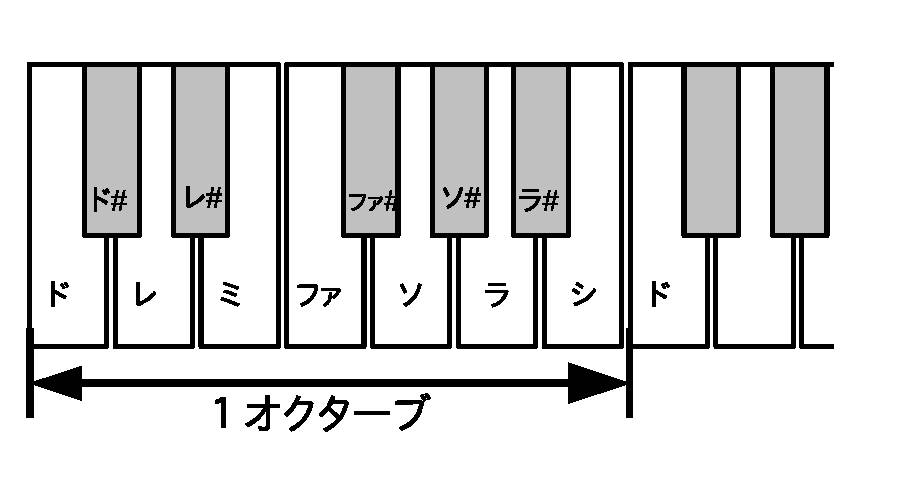
\includegraphics[width=6.2cm]{octave.eps}
    \caption{ピアノの鍵盤}\label{fig:octave}
\end{figure}

さて, 音階を, 周波数が等比数列になるように決めることを, 平均律と呼ぶ。多くの
楽器は平均律で調整されている。以後, 平均律の12音階を考える。
\begin{enumerate}
\item 楽器の調律では, 音階の基準として
周波数440 Hzの「ラ」の音が使われる。この音の2オクターブ上のラ音の
周波数はどのくらいか?
\item 12音階の周波数を等比数列とみたときの公比はどのくらいか?
\item 多くのピアノは, 88個の鍵を持つ。つまり, 88個の音階を出せる。そのような
ピアノの最高音の周波数は, 最低音の周波数の何倍か?
\item 人間耳は, 概ね20Hzから20000Hzまでの音を感じる。その
範囲は何オクターブに相当するか?
\item 上記の範囲をカバーするピアノを作るとしたら, 鍵はいくつ必要か?
\item 基準の「ラ」の音(周波数440 Hz)の, 1.5倍の周波数を持つ音は, 12音階の
中で, どの音階になるか?
\item 1オクターブの中で, ド, ミ, ソのそれぞれの周波数は, およそ4:5:6という
整数比に近い比になることを示せ(これが, ドミソが綺麗な和音になる理由)。
\end{enumerate}
\end{exq}

\begin{exq}\label{q:paper_reflectance} 反射率$r$, 透過率$t$の紙がある。
\begin{enumerate}
\item この紙を2枚かさねたときの反射率を$r$と$t$で表せ。
ヒント: 2枚の紙を, 上から「紙1」「紙2」とする。この2枚重ねの紙に当たった光のうち, 「反射」されるのは, 
\begin{itemize}
\item 紙1の表面で反射される成分。
\item 紙1を透過して紙2の表面で反射し, 紙1を透過する成分。
\item 紙1を透過して紙2の表面で反射し, 紙1の裏面で反射し, 紙2の表面で反射し, 紙1を透過する成分。
\item ...
\end{itemize}
の総和である。
\item 反射率80%, 透過率15%の紙を2枚重ねた時の反射率を求めよ。
\end{enumerate}
\end{exq}

\section*{問題の解答}

\noindent{\textbf{答}}\ref{q:alg_ineq4}  
与式は両辺とも0以上なので, \eref{eq:th_order_9}より, \\左辺$^2 \geq$右辺$^2$を言えばよい。
\begin{eqnarray*} 
&&(\text{左辺})^2-(\text{右辺})^2=\frac{a^2+2ab+b^2}{4}-ab\\
&&=\frac{a^2-2ab+b^2}{4}=\Bigl(\frac{a-b}{2}\Bigr)^2\ge0
\end{eqnarray*}
よって与式は成り立つ。この式で, 等号が成り立つときは$\{(a-b)/2\}^2=0$
なのだから, $(a-b)^2=0$。\eref{eq:ab_0_a_0_b_0}より, $a-b=0$。従って$a=b$。\qed
\mv

\noindent{\textbf{答}}\ref{q:alg_prod0} (1) $4 \cdot 3 \cdot 2 \cdot 1 = 24$  
(2) $5 \cdot 4 \cdot 3 \cdot 2 \cdot 1 = 120$  (3) $1$  (4) $1$  (5) 存在しない。\mv

\noindent{\textbf{答}}\ref{q:alg_comb5} $5!=120$ 通り。
\mv

\noindent{\textbf{答}}\ref{q:alg_comb00} \eref{eq:junretsu}において, $m=n$とすれば, \\
$_n\text{P}_n = n!/(n-n)!=n!/0!=n!$\qed
\mv

\noindent{\textbf{答}}\ref{q:alg_comb0} 8人から3人を選んで順に並べ, その順番で会長・副会長・会計係を割り当てればよい。
つまり, 8人から3人を選ぶ順列だから, $_{8}{\text P}_3 = 336$ 通り。
\mv


\noindent{\textbf{答}}\ref{q:alg_01_8} $2^8=256$通り。
\mv

%\noindent{\textbf{答}}\ref{q:alg_comb2}  
%与式の左辺は, \eref{eq:combination}で$n, m$をそれぞれ$n+1, m+1$とすれば,
%\begin{eqnarray}
%_{n+1}{\text C}_{m+1} & = & \frac{(n+1)!}{(m+1)!\{n+1-(m+1)\}!}\nonumber\\
%                      & = & \frac{(n+1)!}{(m+1)!(n-m)!}\label{eq:sol_alg_comb20}
%\end{eqnarray}
%となる。一方, 与式の右辺第1項は, \eref{eq:combination}で$n, m$をそれぞれ$n, m+1$とすれば, 
%\begin{eqnarray*}
%_{n}{\text C}_{m+1} &=& \frac{n!}{(m+1)!\{n-(m+1)\}!}\\
%                     &=& \frac{n!}{(m+1)!(n-m-1)!}
%\end{eqnarray*}
%となり, 与式の右辺第2項は\eref{eq:combination}をそのまま使えば
%\begin{eqnarray*}
%_{n}{\text C}_{m} =  \frac{n!}{m!(n-m)!}
%\end{eqnarray*}
%となるから, 与式の右辺は, 
%\begin{eqnarray}
%&&_{n}{\text C}_{m+1} +_{n}{\text C}_{m}\nonumber\\
%&& = \frac{n!}{(m+1)!(n-m-1)!} +  \frac{n!}{m!(n-m)!}\nonumber\\
%&& = \frac{n!(n-m)}{(m+1)!(n-m)!}+\frac{n!(m+1)}{(m+1)!(n-m)!}\nonumber\\
%&& = \frac{n!(n-m)+n!(m+1)}{(m+1)!(n-m)!} = \frac{n!(n-m+m+1)}{(m+1)!(n-m)!}\nonumber\\
%&& = \frac{n!(n+1)}{(m+1)!(n-m)!}\nonumber\\
%&& =  \frac{(n+1)!}{(m+1)!(n-m)!}\label{eq:sol_alg_comb21}
%\end{eqnarray}
%となる。\eref{eq:sol_alg_comb20}と\eref{eq:sol_alg_comb21}が等しいから, 
%与式の左辺と右辺は等しい。従って与式が成り立つ\footnote{
%注: この問題は, 以下のように考えることができる。$n+1$人の集団から$m+1$人の
%代表を選ぶとしよう。無論, その選び方は$_{n+1}$C$_{m+1}$通りである。さて, その集団の
%中の特定の一人(ここではAさんと呼ぼう)に着目する。Aさんが代表に入らない場合, 
%その場合の数は, 残り$n$人の中から$m+1$人の代表を選ぶ場合の数になるので, $_n$C$_{m+1}$通り。
%Aさんが代表に入る場合, その場合の数は, 残り$n$人の中から$m$人の代表を選ぶ場合の数になる
%ので, $_n$C$_m$通り。この2パターンで全ての場合を網羅するので, 結局, 与式が成り立つ。}。
%\mv


\noindent{\textbf{答}}\ref{q:alg_comb3} 
(1) 4 (2) 10 (3) 10\\
(4) $n(n-1)(n-2)/6$\\
(5) $_{n}{\text C}_{0}=n!/(0!n!)=n!/n!=1$。ここで$0!=1$を使った。 
(6) 1
\mv

\noindent{\textbf{答}}\ref{q:alg_comb1} 
\eref{eq:combination}より, 
\begin{eqnarray*}
_n{\text C}_m = \frac{n!}{m!\,(n-m)!}
\end{eqnarray*}
一方, \eref{eq:combination}で$m$を$n-m$と置き換えれば, 
\begin{eqnarray*}
_n{\text C}_{n-m} & = & \frac{n!}{(n-m)!\,\{n-(n-m)\}!}\\
                  & = & \frac{n!}{(n-m)!m!} = \frac{n!}{m!(n-m)!}
\end{eqnarray*}
よって, $_n{\text C}_m\,=\,_n{\text C}_{n-m}$ \qed
\mv

\noindent{\textbf{答}}\ref{q:alg_comb4} $_{40}{\text C}_3 = 9880$ 通り。
\mv

\begin{comment}
\noindent{\textbf{答}}\ref{q:alg_poly_tenkai0} 
\begin{edaenumerate}
\item $a^2 + 2ab + b^2$
%\item $a^2 - 2ab +b^2$
%\item $a^3 +3 a^{2} b + 3 a b^{2} + b^3$
\item $a^3 -3 a^{2} b + 3 a b^{2} - b^3$
%\item $a^2 - b^2$
\item $a^3 - b^3$
%\item $a^3 + b^3$
\item $2x^3 + 5x^2 - x - 6$
\end{edaenumerate}
(5) $a^2 + b^2 + c^2 + 2ab + 2bc + 2ca$
\mv
\end{comment}


\noindent{\textbf{答}}\ref{q:alg_poly_tenkai01} $\,\,\,2x^3+3x^2\chi-3x\chi^2-2\chi^3$
\mv

\noindent{\textbf{答}}\ref{q:alg_poly_tenkai2} (1) \eref{eq:binomth}で$a=x$, $b=1$, $n=7$とすれば, 
$(x+1)^7\,=\,_7\text{C}_7\,x^7\,+\,_7\text{C}_6\,x^6\,+\,_7\text{C}_5\,x^5\cdots$
となる。$x^3$の項は, $_7\text{C}_3x^3=35x^3$。従って, 35。 (2) \eref{eq:binomth}で$a=2x$, $b=-3$, $n=6$とすれば, $x^3$の項は
$_6\text{C}_3(2x)^3\times(-3)^3=-4320x^3$。従って, $-4320$。\mv

\begin{comment}
\noindent{\textbf{答}}\ref{q:alg_insu0}  
\begin{edaenumerate}
\item $(a+b)^2$
\item $(a-b)^2$
\item $(a+b)(a^2 - ab + b^2)$
\item $(a-b)(a^2 + ab + b^2)$
\item $(a^2 + b^2)(a+b)(a-b)$
\item $(x-2)(x+1)$
\item $(2x+1)(x-3)$
\item $x(x-1)(x+1)$
\end{edaenumerate}
(9) $x^2=X$とおくと, 与式は,
\begin{eqnarray*}
X^2-5X+4&=&(X-1)(X-4)\\
        &=&(x^2-1)(x^2-4)\\
        &=&(x+1)(x-1)(x+2)(x-2)
\end{eqnarray*}

\noindent{\textbf{答}}\ref{q:alg_wari0}  
\begin{enumerate}
\item 
\begin{eqnarray*}\izyohou{1,1,-1,1}{1,-1}\end{eqnarray*}
従って, 商$x^2 + 2x + 1$,余り$2$
\item 
\begin{eqnarray*}\izyohou{1,2,-1,2,-1}{1,1,1}\end{eqnarray*}
従って, 商$x^2 + x -3$,余り$4x+2$
\end{enumerate}
\hv


\noindent{\textbf{答}}\ref{q:alg_insu3}  
\begin{edaenumerate}
\item $(x-1)(x+2)(x+3)$
\item $(x+1)(x-2)(x+4)$
\end{edaenumerate}
\hv
\end{comment}

\noindent{\textbf{答}}\ref{q:alg_heihokansei0} 
\begin{edaenumerate}<3>
\item \begin{eqnarray*}(x + 2)^2 + 1\end{eqnarray*}
\item \begin{eqnarray*}\Bigl(x + \frac{1}{2}\Bigr)^2 + \frac{3}{4}\end{eqnarray*}
\item \begin{eqnarray*}(x - 1)^2 - 2\end{eqnarray*}
\item \begin{eqnarray*}2(x+1)^2 + 1\end{eqnarray*}
\item \begin{eqnarray*}4\Bigl(x+\frac{1}{8}\Bigr)^2 + \frac{15}{16}\end{eqnarray*}
\end{edaenumerate}
\mv


\noindent{\textbf{答}}\ref{q:alg_eq_insu0} 略解 (レポートではきちんと導出過程を書こう):
(1) $x=-2,3$  (2) $x=1,2$  (3) 左辺を因数分解すると, $(x^2-4)(x^2-1)=(x+2)(x-2)(x+1)(x-1)$。
従って, $x=\pm1, \pm2$
\mv


%\noindent{\textbf{答}}\ref{q:alg_2eq0} 略(誘導に従って計算する。)
%\mv


\noindent{\textbf{答}}\ref{q:alg_eq_complex0} 略解(レポートではきちんと導出過程を書こう):
(1) $x=(-1 \pm \sqrt{7}\,i)/2$ (2) $x=(-3 \pm \sqrt{5})/2$
%\item $x=-1,\, (-1 \pm \sqrt{7}\,i)/2$
%\item $x=1,\, (-1 \pm \sqrt{3}\,i)/2$
%\item $x=\pm 1,\, \pm\, i$
\mv


\noindent{\textbf{答}}\ref{q:alg_series0} (1) $2n -1$ (2) $11 -n$ 
(3) $3^n$ (4) $(1/2)^{n-1}$\mv


% 以下の実数列は, 単調増加するか, 単調減少するか, それともどちらでもないか, 述べよ。
\noindent{\textbf{答}}\ref{q:alg_series1} 
\begin{enumerate}
\item 単調増加。例: $\{1,2,3,4,\cdots\}$
\item 単調減少。例: $\{4,3,2,1,\cdots\}$
\item 単調増加。例: $\{1,2,4,8,\cdots\}$
\item 単調減少。例: $\{-1,-2,-4,-8,\cdots\}$
\item どちらでもない。例: $\{1,-2,4,-8,\cdots\}$
\item 単調減少。例: $\{1,1/2,1/4,1/8,\cdots\}$
\item 単調減少。
\end{enumerate}
\mv


% 以下の実数列は, 収束するか, 発散するか? 収束するならどういう値に収束するか?
\noindent{\textbf{答}}\ref{q:alg_series3} 
\begin{edaenumerate}
<3>
\item 発散($\infty$)
\item 発散($-\infty$)
\item 発散($\infty$)
\item 発散($-\infty$)
\item 0に収束
\item 0に収束
\item 0に収束
\end{edaenumerate}
\mv


\noindent{\textbf{答}}\ref{q:alg_series_sum0} 
\begin{edaenumerate}
\item $2+2+2+2=8$
\item $1+4+9=14$
\item $1+2+4+8=15$
\item $3+5+7+9=24$
\end{edaenumerate}
\mv

\noindent{\textbf{答}}\ref{q:sum_binomth2} 
\begin{eqnarray}
(a+b)^n=\sum_{k=0}^n \,_n\text{C}_k\,a^{n-k}\,b^k
\end{eqnarray}

%\noindent{\textbf{答}}\ref{q:alg_induction_freqmiss} (解答例)\eref{eq:sumk_1}はあくまで$N$で成り立つことを仮定しているだけで, それが$N+1$で成り立つ保証はない。ていうか, それを示すのがそもそもの目的。君は, 示すべき式自体を根拠にしてしまっている。\mv

\noindent{\textbf{答}}\ref{q:alg_series_sum1} 
\begin{enumerate}
\item $n=1$のとき, 与式は, 左辺=$1+r$, 右辺=$1+r$
となるので成り立つ。$n=N$のとき与式が成り立つと仮定する。すなわち, 
\begin{eqnarray}
\sum_{k=0}^N r^k=\frac{1-r^{N+1}}{1-r}\label{eq:sum_touhi_ans2}
\end{eqnarray}
と仮定する。そのとき, 
\begin{eqnarray*}
\sum_{k=0}^{N+1} r^k=\sum_{k=0}^{N} r^k+r^{N+1}=\frac{1-r^{N+1}}{1-r}+r^{N+1}\\
= \frac{1-r^{N+1}+r^{N+1}-r^{N+2}}{1-r} = \frac{1-r^{N+2}}{1-r}
\end{eqnarray*}
となり, $n=N+1$についても与式は成り立つ。\qed
\item $n=1$のとき, 与式は, 左辺=1, 右辺=1となるので成り立つ。
$n=N$のとき与式が成り立つと仮定する。すなわち, 
\begin{eqnarray*}
\sum_{k=1}^N k^2=\frac{N(N+1)(2N+1)}{6}
\end{eqnarray*}
と仮定する。そのとき, 
\begin{eqnarray*}
\sum_{k=1}^{N+1} k^2 & = & \sum_{k=1}^{N} k^2+(N+1)^2\\
        & = & \frac{N(N+1)(2N+1)}{6}+(N+1)^2\\
        & = & \frac{(N+1)\{N(2N+1)+6(N+1)\}}{6}\\
        & = & \frac{(N+1)(2N^2+7N+6)}{6}\\
        & = & \frac{(N+1)(N+2)(2N+3)}{6}
\end{eqnarray*}
これは\eref{eq:sum_xsquare}の右辺で$n$を$N+1$としたものに等しい。従って
与式は$n=N+1$についても成立。
\end{enumerate}

\noindent{\textbf{答}}\ref{q:alg_sum2} 
(1) \eref{eq:sum_touhi}より, $(1-2^{11})/(1-2)=2047$ 
(2) \eref{eq:sum_xsquare}より, $(10\times11\times21)/6=385$

% パソコンの表計算ソフトで, 以下の数列の和を適当に大きな$n$について計算せよ:
%\noindent{\textbf{答}}\ref{q:comp_sum1}  略。
